\hypertarget{sec-technical}{%
\chapter{Advanced Technical Aspects of mlr3}\label{sec-technical}}

\vspace{-15mm}\addtocontents{toc}{\textit{Michel Lang, Sebastian Fischer and Raphael Sonabend}}

\textbf{Michel Lang} \newline  \emph{Research Center Trustworthy Data
Science and Security, and TU Dortmund University}

\textbf{Sebastian Fischer} \newline 
\emph{Ludwig-Maximilians-Universität München, and Munich Center for
Machine Learning (MCML)}

\textbf{Raphael Sonabend} \newline  \emph{Imperial College London}
\newline \newline 

In the previous chapters, we demonstrated how to turn machine learning
concepts and methods into code. In this chapter we will turn to those
technical details that can be important for more advanced uses of
\href{https://mlr3.mlr-org.com}{\texttt{mlr3}}\index{\texttt{mlr3}},
including:

\begin{itemize}
\tightlist
\item
  Parallelization\index{parallelization} with the
  \href{https://cran.r-project.org/package=future}{\texttt{future}}
  framework (Section~\ref{sec-parallelization});
\item
  Error handling and debugging\index{debugging}
  (Section~\ref{sec-error-handling});
\item
  Adjusting the logger to your needs (Section~\ref{sec-logging});
\item
  Working with out-of-memory data, e.g., data stored in databases
  (Section~\ref{sec-backends}); and
\item
  Adding new classes to \texttt{mlr3} (Section~\ref{sec-extending}).
\end{itemize}

\hypertarget{sec-parallelization}{%
\section{Parallelization}\label{sec-parallelization}}

The term parallelization\index{parallelization} refers to running
multiple algorithms in parallel, i.e., executing them simultaneously on
multiple CPU cores, CPUs, or computational nodes. Not all algorithms can
be parallelized, but when they can, parallelization allows significant
savings in computation time.

In general, there are many possibilities to parallelize, depending on
the hardware to run the computations. If you only have a single CPU with
multiple cores, then \emph{threads} or \emph{processes} are ways to
utilize all cores on a local machine. If you have multiple machines on
the other hand, they can communicate and exchange information via
protocols such as \emph{network sockets} or the \emph{Message Passing
Interface}. Larger computational sites rely on scheduling systems to
orchestrate the computation for multiple users and usually offer a
shared network file system all machines can access. Interacting with
scheduling systems on compute clusters is covered in
Section~\ref{sec-hpc-exec} using the R package
\href{https://cran.r-project.org/package=batchtools}{\texttt{batchtools}}.

There are a few pieces of terminology associated with parallelization
that we will use in this section:

\begin{itemize}
\tightlist
\item
  The parallelization
  backend\index{parallelization backend}{\marginnote{\begin{footnotesize}Parallelization
  Backend\end{footnotesize}}} is the hardware to parallelize with a
  respective interface provided by an R package. Many parallelization
  backends have different APIs, so we use the
  \href{https://cran.r-project.org/package=future}{\texttt{future}}
  package as a unified, abstraction layer for many parallelization
  backends. From a user perspective, \texttt{mlr3} interfaces with
  \texttt{future} directly so all you will need to do is configure the
  backend before starting any computations.
\item
  The Main process is the R session or process that orchestrates the
  computational work, called jobs.
\item
  Workers are the R sessions, processes, or machines that receive the
  jobs, perform calculations, and then send the results back to Main.
\end{itemize}

An important step in parallel programming involves the identification of
sections of the program flow that are both time-consuming
(`bottlenecks') and can run independently of a different section, i.e.,
section A's operations are not dependent on the results of section B's
operations, and vice versa. Fortunately, these sections are usually
relatively easy to spot for machine learning experiments:

\begin{enumerate}
\def\labelenumi{\arabic{enumi}.}
\tightlist
\item
  Training of a learning algorithm (or other computationally intensive
  parts of a machine learning pipeline) \emph{may} contain independent
  sections which can run in parallel, e.g.

  \begin{itemize}
  \tightlist
  \item
    A single decision tree\index{decision tree} iterates over all
    features to find the best split point, for each feature
    independently.
  \item
    A random forest\index{random forest} usually fits hundreds of trees
    independently.
  \end{itemize}

  The key principle that makes parallelization possible for these
  examples (and in general in many fields of statistics and ML) is
  called data
  parallelism\index{data parallelism}{\marginnote{\begin{footnotesize}Data
  Parallelism\end{footnotesize}}}, which means the same operation is
  performed concurrently on different elements of the input data.
  Parallelization of learning algorithms is covered in
  Section~\ref{sec-parallel-learner}.
\item
  Resampling consists of independent repetitions of train-test-splits
  and benchmarking consists of multiple independent resamplings
  (Section~\ref{sec-parallel-resample}).
\item
  Tuning (Chapter~\ref{sec-optimization}) often is iterated
  benchmarking, embedded in a sequential procedure that determines the
  hyperparameter configurations to try next. While many tuning
  algorithms are inherently sequential to some degree, there are some
  (e.g., random search) that can propose multiple configurations in
  parallel to be evaluated independently, providing another level for
  parallelization (Section~\ref{sec-nested-resampling-parallelization}).
\item
  Predictions of a single learner for multiple observations can be
  computed independently (Section~\ref{sec-parallel-predict}).
\end{enumerate}

These examples are referred to as ``embarrassingly
parallel\index{embarrassingly parallel}{\marginnote{\begin{footnotesize}Embarrassingly
Parallel\end{footnotesize}}}'' as they are so easy to parallelize. If we
can formulate the problem as a function that can be passed to map-like
functions such as
\href{https://www.rdocumentation.org/packages/base/topics/lapply}{\texttt{lapply()}},
then you have an embarrassingly parallel problem. However, just because
a problem \emph{can} be parallelized, it does not follow that every
operation in a problem \emph{should} be parallelized. Starting and
terminating workers as well as possible communication between workers
comes at a price in the form of additionally required runtime which is
called parallelization
overhead\index{parallelization overhead}{\marginnote{\begin{footnotesize}Parallelization
Overhead\end{footnotesize}}}. This overhead strongly varies between
parallelization backends and must be carefully weighed against the
runtime of the sequential execution to determine if parallelization is
worth the effort. If the sequential execution is comparably fast,
enabling parallelization may introduce additional complexity with little
runtime savings, or could even slow down the execution. It is possible
to control the
granularity\index{granularity}{\marginnote{\begin{footnotesize}Granularity\end{footnotesize}}}
of the parallelization to reduce the parallelization overhead. For
example, we could reduce the overhead of parallelizing a
\texttt{for}-loop with 1000 iterations on four CPU cores by
chunking\index{chunking} the work of the 1000 jobs into four
computational jobs performing 250 iterations each, resulting in four big
jobs and not 1000 small ones.

This effect is illustrated in the following code chunk using a socket
cluster\index{socket cluster} with the
\href{https://cran.r-project.org/package=parallel}{\texttt{parallel}}
package, which has a \texttt{chunk.size} option so we do not need to
manually create chunks:

\begin{Shaded}
\begin{Highlighting}[]
\CommentTok{\# set up a socket cluster with 4 workers on the local machine}
\FunctionTok{library}\NormalTok{(parallel)}
\NormalTok{cores }\OtherTok{=} \DecValTok{4}
\NormalTok{cl }\OtherTok{=} \FunctionTok{makeCluster}\NormalTok{(cores)}

\CommentTok{\# vector to operate on}
\NormalTok{x }\OtherTok{=} \DecValTok{1}\SpecialCharTok{:}\DecValTok{10000}

\CommentTok{\# fast function to parallelize}
\NormalTok{f }\OtherTok{=} \ControlFlowTok{function}\NormalTok{(y) }\FunctionTok{sqrt}\NormalTok{(y }\SpecialCharTok{+} \DecValTok{1}\NormalTok{)}

\CommentTok{\# unchunked approach: 1000 jobs}
\FunctionTok{system.time}\NormalTok{(\{}\FunctionTok{parSapply}\NormalTok{(cl, x, f, }\AttributeTok{chunk.size =} \DecValTok{1}\NormalTok{)\})}
\end{Highlighting}
\end{Shaded}

\begin{verbatim}
   user  system elapsed 
  0.504   0.120   0.780 
\end{verbatim}

\begin{Shaded}
\begin{Highlighting}[]
\CommentTok{\# chunked approach: 4 jobs}
\FunctionTok{system.time}\NormalTok{(\{}\FunctionTok{parSapply}\NormalTok{(cl, x, f, }\AttributeTok{chunk.size =} \DecValTok{2500}\NormalTok{)\})}
\end{Highlighting}
\end{Shaded}

\begin{verbatim}
   user  system elapsed 
  0.003   0.001   0.013 
\end{verbatim}

Whenever you have the option to control the granularity by setting the
chunk size, you should aim for at least as many jobs as workers.
However, if there are too few job chunks with strongly dissimilar
runtimes, the system may end up waiting for the last chunk to finish,
while other resources are idle. This is referred to as synchronization
overhead\index{synchronization overhead}{\marginnote{\begin{footnotesize}Synchronization
Overhead\end{footnotesize}}}. You should therefore aim for chunks with a
runtime of at least several seconds, so that the parallelization
overhead remains reasonable, while still having enough chunks to ensure
that you can fully utilize the system. If you have heterogeneous
runtimes, you can consider grouping jobs so that the runtimes of the
chunks are more homogeneous. If runtimes can be estimated, then both
\texttt{batchtools::binpack()} and \texttt{batchtools::lpt()}
(documented together with the
\href{https://www.rdocumentation.org/packages/batchtools/topics/chunk}{\texttt{chunk()}}
function) are useful for chunking jobs. If runtimes cannot be estimated,
then it can be useful to randomize the order of jobs. Otherwise jobs
could be accidentally ordered by runtime, for example because they are
sorted by a hyperparameter that has a strong influence on training time.
Naively chunking jobs could then lead to some chunks containing much
more expensive jobs than others, resulting in avoidable underutilization
of resources.
\href{https://mlr3misc.mlr-org.com}{\texttt{mlr3misc}}\index{\texttt{mlr3misc}}
ships with the functions
\href{https://mlr3misc.mlr-org.com/reference/chunk.html}{\texttt{chunk()}}
and
\href{https://mlr3misc.mlr-org.com/reference/chunk_vector.html}{\texttt{chunk\_vector()}}
that conveniently chunk jobs and also shuffle them by default. There are
also options to control the chunk size for parallelization in
\texttt{mlr3}, which are discussed in
Section~\ref{sec-parallel-resample}.

\begin{tcolorbox}[enhanced jigsaw, opacitybacktitle=0.6, rightrule=.15mm, opacityback=0, arc=.35mm, breakable, titlerule=0mm, colframe=quarto-callout-tip-color-frame, coltitle=black, bottomrule=.15mm, toprule=.15mm, colback=white, colbacktitle=quarto-callout-tip-color!10!white, bottomtitle=1mm, toptitle=1mm, title=\textcolor{quarto-callout-tip-color}{\faLightbulb}\hspace{0.5em}{Reproducibility}, leftrule=.75mm, left=2mm]

Reproducibility is often a concern during parallelization because
special Pseudorandom number generators (PRNGs) may be required
(Bengtsson 2020). However,
\href{https://cran.r-project.org/package=future}{\texttt{future}}
ensures that all workers will receive the same PRNG streams, independent
of the number of workers (Bengtsson 2020). Therefore, \texttt{mlr3}
experiments will be reproducible as long as you use \texttt{set.seed} at
the start of your scripts (with the PRNG of your choice).

\end{tcolorbox}

\hypertarget{sec-parallel-learner}{%
\subsection{Parallelization of Learners}\label{sec-parallel-learner}}

At the lowest level, external code can be parallelized if available in
underlying implementations. For example, while fitting a single decision
tree, each split that divides the data into two disjoint partitions
requires a search for the best cut point on all \(p\) features. Instead
of iterating over all features sequentially, the search can be broken
down into \(p\) threads, each searching for the best cut point on a
single feature. These threads can then be scheduled depending on
available CPU cores, as there is no need for communication between the
threads. After all the threads have finished, the results are collected
and merged before terminating the threads. The \(p\) best-cut points per
feature are collected and aggregated to the single best-cut point across
all features by iterating over the \(p\) results sequentially.

\begin{tcolorbox}[enhanced jigsaw, opacitybacktitle=0.6, rightrule=.15mm, opacityback=0, arc=.35mm, breakable, titlerule=0mm, colframe=quarto-callout-tip-color-frame, coltitle=black, bottomrule=.15mm, toprule=.15mm, colback=white, colbacktitle=quarto-callout-tip-color!10!white, bottomtitle=1mm, toptitle=1mm, title=\textcolor{quarto-callout-tip-color}{\faLightbulb}\hspace{0.5em}{GPU Computation}, leftrule=.75mm, left=2mm]

Parallelization on GPUs is not covered in this book. \texttt{mlr3} only
distributes the fitting of multiple learners, e.g., during resampling,
benchmarking, or tuning. On this rather abstract level, GPU
parallelization does not work efficiently. However, some learning
procedures can be compiled against CUDA/OpenCL to utilize the GPU while
fitting a single model. We refer to the respective documentation of the
learner's implementation, e.g.,
\url{https://xgboost.readthedocs.io/en/stable/gpu/} for XGBoost.

\end{tcolorbox}

Threading\index{threading} is implemented in the compiled code of the
package (e.g., in C or C++), which means that the R interpreter calls
the external code and waits for the results to be returned, without
noticing that the computations are executed in parallel. Therefore,
threading can conflict with certain parallel backends, leading the
system to be overutilized in the best-case scenario, or causing hangs or
segfaults in the worst case. For this reason, we introduced the
convention that threading parallelization is turned off by default.
Hyperparameters that control the number of threads are tagged with the
label \texttt{"threads"}:

\begin{Shaded}
\begin{Highlighting}[]
\NormalTok{lrn\_ranger }\OtherTok{=} \FunctionTok{lrn}\NormalTok{(}\StringTok{"classif.ranger"}\NormalTok{)}

\CommentTok{\# show all hyperparameters tagged with "threads"}
\NormalTok{lrn\_ranger}\SpecialCharTok{$}\NormalTok{param\_set}\SpecialCharTok{$}\FunctionTok{ids}\NormalTok{(}\AttributeTok{tags =} \StringTok{"threads"}\NormalTok{)}
\end{Highlighting}
\end{Shaded}

\begin{verbatim}
[1] "num.threads"
\end{verbatim}

\begin{Shaded}
\begin{Highlighting}[]
\CommentTok{\# The number of threads is initialized to 1}
\NormalTok{lrn\_ranger}\SpecialCharTok{$}\NormalTok{param\_set}\SpecialCharTok{$}\NormalTok{values}\SpecialCharTok{$}\NormalTok{num.threads}
\end{Highlighting}
\end{Shaded}

\begin{verbatim}
[1] 1
\end{verbatim}

To enable the parallelization for this learner, \texttt{mlr3} provides
the helper function
\href{https://mlr3.mlr-org.com/reference/set_threads.html}{\texttt{set\_threads()}},
which automatically adjusts the hyperparameters associated with builtin
learner parallelization:

\begin{Shaded}
\begin{Highlighting}[]
\CommentTok{\# use four CPUs}
\FunctionTok{set\_threads}\NormalTok{(lrn\_ranger, }\AttributeTok{n =} \DecValTok{4}\NormalTok{)}
\end{Highlighting}
\end{Shaded}

\begin{verbatim}
<LearnerClassifRanger:classif.ranger>
* Model: -
* Parameters: num.threads=4
* Packages: mlr3, mlr3learners, ranger
* Predict Types:  [response], prob
* Feature Types: logical, integer, numeric, character, factor,
  ordered
* Properties: hotstart_backward, importance, multiclass,
  oob_error, twoclass, weights
\end{verbatim}

If we did not specify an argument for the \texttt{n} parameter then the
default is a heuristic to detect the correct number using
\href{https://www.rdocumentation.org/packages/parallelly/topics/availableCores}{\texttt{availableCores()}}.
This heuristic is not always ideal (interested readers might want to
look up ``Amdahl's Law'') and utilizing all available cores is
occasionally counterproductive and can slow down overall runtime
(Bengtsson 2022), moreover using all cores is not ideal if:

\begin{itemize}
\tightlist
\item
  You want to simultaneously use your system for other purposes.
\item
  You are on a multi-user system and want to spare some resources for
  other users.
\item
  You have linked R to a threaded BLAS\index{BLAS} implementation like
  OpenBLAS and your learners make heavy use of linear algebra.
\end{itemize}

\begin{Shaded}
\begin{Highlighting}[]
\CommentTok{\# auto{-}detect cores on the local machine}
\FunctionTok{set\_threads}\NormalTok{(lrn\_ranger)}
\end{Highlighting}
\end{Shaded}

\begin{verbatim}
<LearnerClassifRanger:classif.ranger>
* Model: -
* Parameters: num.threads=8
* Packages: mlr3, mlr3learners, ranger
* Predict Types:  [response], prob
* Feature Types: logical, integer, numeric, character, factor,
  ordered
* Properties: hotstart_backward, importance, multiclass,
  oob_error, twoclass, weights
\end{verbatim}

To control how many cores are set, we recommend manually setting the
number of CPUs in your system's \texttt{.Rprofile} file:

\begin{Shaded}
\begin{Highlighting}[]
\FunctionTok{options}\NormalTok{(}\AttributeTok{mc.cores =} \DecValTok{4}\NormalTok{)}
\end{Highlighting}
\end{Shaded}

There are also other approaches for parallelization of learners, e.g.~by
directly supporting one specific parallelization backend or a
parallelization framework like
\href{https://cran.r-project.org/package=foreach}{\texttt{foreach}}. If
this is supported, parallelization must be explicitly activated, e.g.~by
setting a hyperparameter. If you need to parallelize on the learner
level because a single model fit takes too much time, and you only fit a
few of these models, consult the documentation of the respective
learner. In many scenarios, it makes more sense to parallelize on a
different level like resampling or benchmarking which is covered in the
following subsections.

\hypertarget{sec-parallel-resample}{%
\subsection{Parallelization of Resamplings and
Benchmarks}\label{sec-parallel-resample}}

In addition to parallel learners, most machine learning experiments can
be easily parallelized during resampling. By definition, resampling is
performed by aggregating over independent repetitions of multiple
train-test splits.

\texttt{mlr3} makes use of
\href{https://cran.r-project.org/package=future}{\texttt{future}} to
enable parallelization over resampling iterations using the parallel
backend, which can be configured by the user via the
\href{https://www.rdocumentation.org/packages/future/topics/plan}{\texttt{plan()}}
function.

By example, we will look at parallelizing three-fold CV for a decision
tree on the sonar task (Figure~\ref{fig-parallel-overview}). We use the
\href{https://www.rdocumentation.org/packages/future/topics/multisession}{\texttt{multisession}}
plan (which internally uses socket clusters from the \texttt{parallel}
package) that should work on all operating systems.

\begin{Shaded}
\begin{Highlighting}[]
\FunctionTok{library}\NormalTok{(future)}

\CommentTok{\# select the multisession backend to use}
\NormalTok{future}\SpecialCharTok{::}\FunctionTok{plan}\NormalTok{(}\StringTok{"multisession"}\NormalTok{)}

\CommentTok{\# run our experiment}
\NormalTok{tsk\_sonar }\OtherTok{=} \FunctionTok{tsk}\NormalTok{(}\StringTok{"sonar"}\NormalTok{)}
\NormalTok{lrn\_rpart }\OtherTok{=} \FunctionTok{lrn}\NormalTok{(}\StringTok{"classif.rpart"}\NormalTok{)}
\NormalTok{rsmp\_cv3 }\OtherTok{=} \FunctionTok{rsmp}\NormalTok{(}\StringTok{"cv"}\NormalTok{, }\AttributeTok{folds =} \DecValTok{3}\NormalTok{)}
\FunctionTok{system.time}\NormalTok{(\{}\FunctionTok{resample}\NormalTok{(tsk\_sonar, lrn\_rpart, rsmp\_cv3)\})}
\end{Highlighting}
\end{Shaded}

\begin{verbatim}
   user  system elapsed 
  0.068   0.003   0.481 
\end{verbatim}

By default, all CPUs of your machine are used unless you specify the
argument \texttt{workers} in \texttt{future::plan()} (see the previous
section for issues that this might cause). In contrast to threads, the
technical overhead for starting workers, communicating objects, sending
back results, and shutting down the workers is quite large for the
\texttt{"multisession"} backend.

The
\href{https://www.rdocumentation.org/packages/future/topics/multicore}{\texttt{multicore}}
backend comes with more overhead than threading, but considerably less
overhead than \texttt{"multisession"}, as the \texttt{"multicore"}
backend only copies R objects when modified (`copy-on-write'), whereas
objects are always copied to the respective session before any
computation for \texttt{"multisession"}. The \texttt{"multicore"}
backend has the major disadvantage that it is not supported on Windows
systems - for this reason, we will stick with the
\texttt{"multisession"} backend for all examples here.

In general, it is advised to only consider parallelization for
resamplings where each iteration runs at least a few seconds. There are
two \texttt{mlr3} options to control the execution and granularity:

\begin{itemize}
\tightlist
\item
  If \texttt{mlr3.exec\_random} is set to \texttt{TRUE} (default), the
  order of jobs is randomized in resamplings and benchmarks. This can
  help if you run a benchmark or tuning with heterogeneous runtimes.
\item
  Option \texttt{mlr3.exec\_chunk\_size} can be used to control how many
  jobs are mapped to a single \texttt{future} and defaults to
  \texttt{1}. The value of this option is passed to
  \href{https://www.rdocumentation.org/packages/future.apply/topics/future_mapply}{\texttt{future\_mapply()}}
  and \texttt{future.scheduling} is constantly set to \texttt{TRUE}.
\end{itemize}

Tuning the chunk size can help in some rare cases to mitigate the
parallelization overhead but is unlikely to be useful in larger problems
or longer runtimes.

\begin{figure}

{\centering 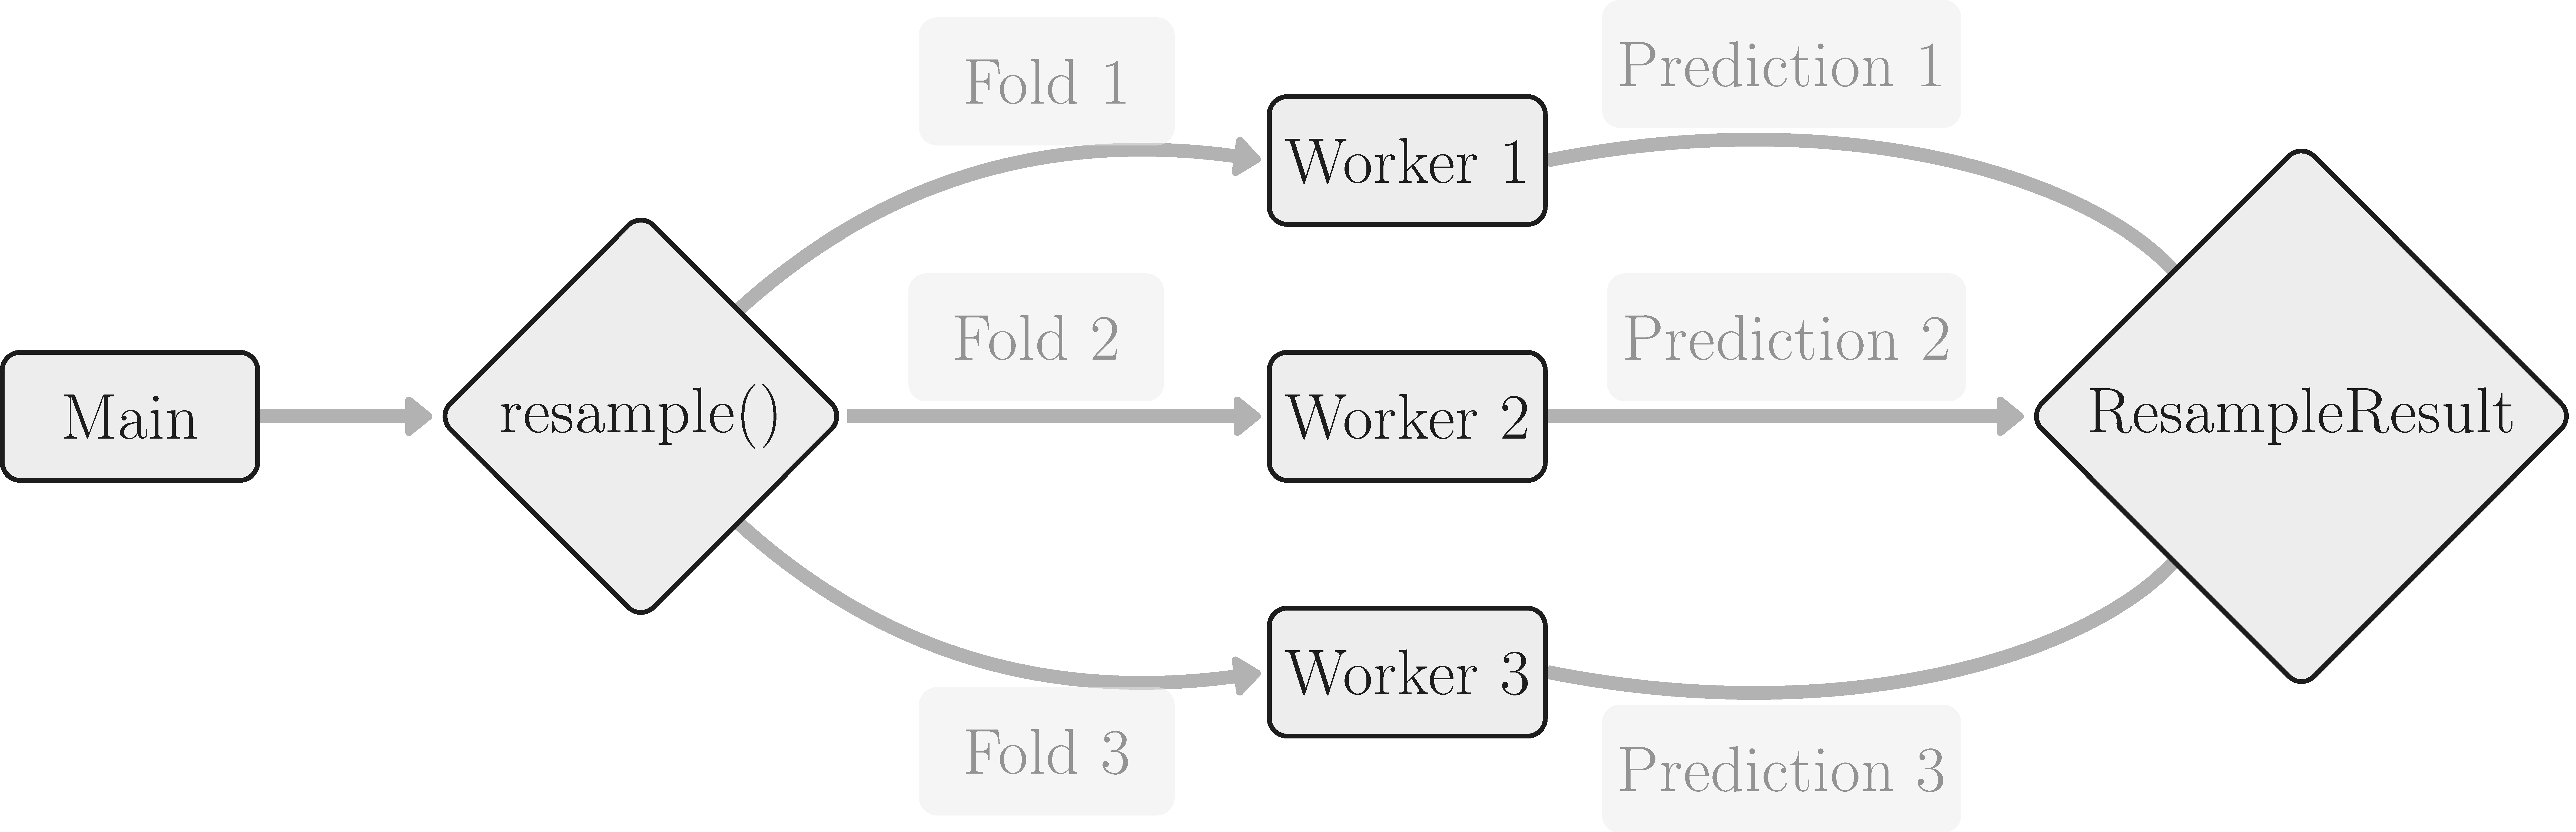
\includegraphics[width=1\textwidth,height=\textheight]{chapters/chapter10/Figures/mlr3book_figures-30.png}

}

\caption{\label{fig-parallel-overview}Parallelization of a resampling
using three-fold CV. The main process calls the \texttt{resample()}
function, which starts the parallelization process and the computational
task is split into three parts for three-fold CV. The folds are passed
to three workers, each fitting a model on the respective subset of the
task and predicting on the left-out observations. The predictions (and
trained models) are communicated back to the main process which combines
them into a \texttt{ResampleResult}.}

\end{figure}

Benchmarks\index{benchmark experiments} can be seen as a collection of
multiple independent resamplings where a combination of a task, a
learner, and a resampling strategy defines one resampling to perform. In
pseudo-code, the calculation can be written as

\begin{verbatim}
foreach combination of (task, learner, resampling strategy) {
    foreach resampling iteration {
        execute(resampling, j)
    }
}
\end{verbatim}

Therefore we could either:

\begin{enumerate}
\def\labelenumi{\arabic{enumi}.}
\tightlist
\item
  Parallelize over all resamplings and execute each resampling
  sequentially (parallelize outer loop); or
\item
  Iterate over all resamplings and execute each resampling in parallel
  (parallelize inner loop).
\end{enumerate}

\texttt{mlr3} simplifies this decision for you by flattening all
experiments to the same level, i.e.,
\href{https://mlr3.mlr-org.com/reference/benchmark.html}{\texttt{benchmark()}}
iterates over the elements of the Cartesian product of the iterations of
the outer and inner loops. Therefore, there is no need to decide whether
you want to parallelize the tuning \emph{or} the resampling, you always
parallelize both. This approach makes the computation fine-grained and
allows the \texttt{future} backend to group the jobs into chunks of
suitable size (depending on the number of workers), it also makes the
procedure identical to parallelizing resampling:

\begin{Shaded}
\begin{Highlighting}[]
\CommentTok{\# simple benchmark design}
\NormalTok{design }\OtherTok{=} \FunctionTok{benchmark\_grid}\NormalTok{(}\FunctionTok{tsks}\NormalTok{(}\FunctionTok{c}\NormalTok{(}\StringTok{"sonar"}\NormalTok{, }\StringTok{"penguins"}\NormalTok{)),}
  \FunctionTok{lrns}\NormalTok{(}\FunctionTok{c}\NormalTok{(}\StringTok{"classif.featureless"}\NormalTok{, }\StringTok{"classif.rpart"}\NormalTok{)), rsmp\_cv3)}

\CommentTok{\# enable parallelization}
\NormalTok{future}\SpecialCharTok{::}\FunctionTok{plan}\NormalTok{(}\StringTok{"multisession"}\NormalTok{)}

\CommentTok{\# run benchmark in parallel}
\NormalTok{bmr }\OtherTok{=} \FunctionTok{benchmark}\NormalTok{(design)}
\end{Highlighting}
\end{Shaded}

See Section~\ref{sec-hpc-exec} for larger benchmark experiments that may
have a cumulative runtime of weeks, months or even years.

\hypertarget{sec-parallel-tuning}{%
\subsection{Parallelization of Tuning}\label{sec-parallel-tuning}}

Tuning is usually an iterative procedure, consisting of steps that are
themselves embarrassingly parallel. In each iteration, a tuner proposes
a batch of hyperparameter configurations (which could be of size
\texttt{1}), which can then be evaluated in parallel. After each
iteration, most tuners adapt themselves in some way based on the
obtained performance values. Random and grid search are exceptions as
they do not choose configurations based on past results, instead, for
these tuners, all evaluations are independent and can, in principle, be
fully parallelized.

Tuning is implemented in \texttt{mlr3} as iterative benchmarks. The
\href{https://mlr3tuning.mlr-org.com/reference/Tuner.html}{\texttt{Tuner}}
proposes a batch of learners, each with a different configuration in its
\texttt{\$param\_set\$values}, where the size of the batch can usually
be controlled with the \texttt{batch\_size} configuration parameter.
This batch is passed to
\href{https://mlr3.mlr-org.com/reference/benchmark.html}{\texttt{benchmark()}}
with the resampling strategy of the tuning instance.

Since each call to \texttt{benchmark()} depends on previous results, it
is generally not possible to parallelize tuning at a higher ``level''
than individual benchmarks. Instead, the individual \texttt{benchmark()}
evaluations are parallelized by \texttt{mlr3} as if they were
experiments without tuning. This means that the individual resampling
iterations of each evaluated configuration are all parallelized at the
same time. To ensure full parallelization, make sure that the
\texttt{batch\_size} multiplied by the number of resampling iterations
is at least equal to the number of available workers. If you expect
homogeneous runtimes, i.e., you are tuning over a single learner or
pipeline without any hyperparameters with a large influence on the
runtime, aim for a multiple of the number of workers. In general, larger
batches allow for more parallelization, while smaller batches imply a
more frequent evaluation of the termination criteria. Independently of
whether you use parallelization, the termination criteria are only
checked between evaluations of batches.

The following code shows a parallelized execution of random search with
the termination criterion set to 20 iterations and a moderate batch
size, where 36 resampling splits -- 12 configurations of three splits
each -- are evaluated in parallel on four workers. The batch size, set
to a multiple of the number of workers, ensures that available resources
are used efficiently. However, note that the tuning only terminates
after a multiple of the given batch size, in this case after 24
evaluations.

\begin{Shaded}
\begin{Highlighting}[]
\NormalTok{future}\SpecialCharTok{::}\FunctionTok{plan}\NormalTok{(}\StringTok{"multisession"}\NormalTok{, }\AttributeTok{workers =} \DecValTok{4}\NormalTok{)}

\NormalTok{instance }\OtherTok{=} \FunctionTok{tune}\NormalTok{(}
  \FunctionTok{tnr}\NormalTok{(}\StringTok{"random\_search"}\NormalTok{, }\AttributeTok{batch\_size =} \DecValTok{12}\NormalTok{),}
  \FunctionTok{tsk}\NormalTok{(}\StringTok{"penguins"}\NormalTok{),}
  \FunctionTok{lrn}\NormalTok{(}\StringTok{"classif.rpart"}\NormalTok{, }\AttributeTok{minsplit =} \FunctionTok{to\_tune}\NormalTok{(}\DecValTok{2}\NormalTok{, }\DecValTok{128}\NormalTok{)),}
  \FunctionTok{rsmp}\NormalTok{(}\StringTok{"cv"}\NormalTok{, }\AttributeTok{folds =} \DecValTok{3}\NormalTok{),}
  \AttributeTok{term\_evals =} \DecValTok{20}
\NormalTok{)}

\NormalTok{instance}\SpecialCharTok{$}\NormalTok{archive}\SpecialCharTok{$}\NormalTok{n\_evals}
\end{Highlighting}
\end{Shaded}

\begin{verbatim}
[1] 24
\end{verbatim}

In this example, we could have increased the batch size to 20 to make
use of available resources in the most efficient way while stopping
exactly at the number of evaluations, however this does not generalize
to other termination criteria where we do not know the number of
evaluations in advance. For example, if we used
\texttt{trm("perf\_reached")} with a batch size of 12, then if the first
configuration of the batch yielded better performance than the given
threshold, the remaining 11 configurations would still be unnecessarily
evaluated.

\hypertarget{sec-nested-resampling-parallelization}{%
\subsection{Nested Resampling
Parallelization}\label{sec-nested-resampling-parallelization}}

Nested resampling can conceptually be parallelized at three different
levels, each corresponding to jobs of different granularity:

\begin{enumerate}
\def\labelenumi{\arabic{enumi}.}
\tightlist
\item
  The parallelization of the outer resampling. A job is then the tuning
  of a learner on the respective training set of the outer resampling
  splits.
\item
  The parallel evaluation of the batch of hyperparameter configurations
  proposed in one tuning iteration. A job is then, for example, the
  cross-validation of such a configuration.
\item
  The parallelization of the inner resampling in tuning. A job is then a
  train-predict-score step of a single configuration.
\end{enumerate}

This is demonstrated in the pseudocode below, which is a simplified form
of Algorithm 3 from Bischl et al. (2023):

\begin{Shaded}
\begin{Highlighting}[]
\CommentTok{\# outer resampling, level 1:}
\ControlFlowTok{for}\NormalTok{ (i }\ControlFlowTok{in} \FunctionTok{seq\_len}\NormalTok{(n\_outer\_splits)) \{}
  \CommentTok{\# tuning instance, in this example mainly represents the archive}
\NormalTok{  tuning\_inst }\OtherTok{=} \FunctionTok{ti}\NormalTok{(...)}
\NormalTok{  inner\_task }\OtherTok{=} \FunctionTok{get\_training\_task}\NormalTok{(task, outer\_splits[[i]])}
  \CommentTok{\# tuning loop, the details of which depend on the tuner being used}
  \CommentTok{\# This does not correspond to a level:}
  \ControlFlowTok{while}\NormalTok{ (}\SpecialCharTok{!}\NormalTok{tuning\_inst}\SpecialCharTok{$}\NormalTok{is\_terminated) \{}
\NormalTok{    proposed\_points }\OtherTok{=} \FunctionTok{propose\_points}\NormalTok{(tuning\_inst}\SpecialCharTok{$}\NormalTok{archive, batch\_size)}
    \CommentTok{\# Evaluation of configurations, level 2:}
    \ControlFlowTok{for}\NormalTok{ (hp\_configuration }\ControlFlowTok{in}\NormalTok{ proposed\_points) \{}
\NormalTok{      split\_performances }\OtherTok{=} \FunctionTok{numeric}\NormalTok{()}
      \CommentTok{\# Inner resampling, level 3:}
      \ControlFlowTok{for}\NormalTok{ (j }\ControlFlowTok{in} \FunctionTok{seq\_len}\NormalTok{(n\_inner\_splits)) \{}
\NormalTok{        split\_performances[j] }\OtherTok{=} \FunctionTok{evaluate\_performance}\NormalTok{(}
\NormalTok{          learner, hp\_configuration, inner\_task, inner\_splits[[j]]}
\NormalTok{        )}
\NormalTok{      \}}
\NormalTok{      performance }\OtherTok{=} \FunctionTok{aggregate}\NormalTok{(split\_performances)}
      \FunctionTok{update\_archive}\NormalTok{(tuning\_inst}\SpecialCharTok{$}\NormalTok{archive, configuration, performance)}
\NormalTok{    \}}
\NormalTok{  \}}
  \FunctionTok{evaluate\_performance}\NormalTok{(}
\NormalTok{    learner, tuning\_inst}\SpecialCharTok{$}\NormalTok{result, task, outer\_splits[[i]]}
\NormalTok{  )}
\NormalTok{\}}
\end{Highlighting}
\end{Shaded}

This algorithm is implemented in \texttt{mlr3} in a slightly more
efficient manner. At the second level (the evaluation of hyperparameter
configurations), it exploits the functionality of \texttt{benchmark()}:
a \texttt{Learner} object is created for each proposed hyperparameter
configuration and all learners are resampled in a benchmark experiment
in the innermost for-loop, effectively executing the second level along
with the third level on a finer granularity (number of proposed points
times number of inner resampling iterations). Hence, when parallelizing
nested resampling in \texttt{mlr3}, the user only has to choose between
two options: parallelizing the outer resampling or the inner
benchmarking.

By example, let us tune the \texttt{minsplit} argument of a
classification tree using an
\href{https://mlr3tuning.mlr-org.com/reference/AutoTuner.html}{\texttt{AutoTuner}}
(Section~\ref{sec-autotuner}) and random search with only two
iterations. Note that this is a didactic example to illustrate the
interplay of the different parallelization levels and not a realistic
setup. We use holdout for inner resampling and set the
\texttt{batch\_size} to \texttt{2}, which yields two independent
iterations in the inner benchmark experiment. A five-fold CV is used for
our outer resampling. For the sake of simplicity, we will also ignore
the final model fit the \texttt{AutoTuner} performs after tuning. Below,
we run the example sequentially without parallelization:

\begin{Shaded}
\begin{Highlighting}[]
\FunctionTok{library}\NormalTok{(mlr3tuning)}
\CommentTok{\# reset to default sequential plan}
\NormalTok{future}\SpecialCharTok{::}\FunctionTok{plan}\NormalTok{(}\StringTok{"sequential"}\NormalTok{)}

\NormalTok{lrn\_rpart }\OtherTok{=} \FunctionTok{lrn}\NormalTok{(}\StringTok{"classif.rpart"}\NormalTok{,}
  \AttributeTok{minsplit  =} \FunctionTok{to\_tune}\NormalTok{(}\DecValTok{2}\NormalTok{, }\DecValTok{128}\NormalTok{))}

\NormalTok{lrn\_rpart\_tuned }\OtherTok{=} \FunctionTok{auto\_tuner}\NormalTok{(}\FunctionTok{tnr}\NormalTok{(}\StringTok{"random\_search"}\NormalTok{, }\AttributeTok{batch\_size =} \DecValTok{2}\NormalTok{),}
\NormalTok{  lrn\_rpart, }\FunctionTok{rsmp}\NormalTok{(}\StringTok{"holdout"}\NormalTok{), }\FunctionTok{msr}\NormalTok{(}\StringTok{"classif.ce"}\NormalTok{), }\DecValTok{2}\NormalTok{)}

\NormalTok{rr }\OtherTok{=} \FunctionTok{resample}\NormalTok{(}\FunctionTok{tsk}\NormalTok{(}\StringTok{"penguins"}\NormalTok{), lrn\_rpart\_tuned, }\FunctionTok{rsmp}\NormalTok{(}\StringTok{"cv"}\NormalTok{, }\AttributeTok{folds =} \DecValTok{5}\NormalTok{))}
\end{Highlighting}
\end{Shaded}

We can now either opt to parallelize the outer CV or the inner
benchmarking. Let us assume we have a single CPU with four cores (C1 -
C4) available and each inner holdout evaluation during tuning takes four
seconds. If we parallelize the outer five-fold CV
(Figure~\ref{fig-parallel-outer}), each of the four cores would run one
outer resampling first, the computation of the fifth iteration has to
wait as there are no more available cores.

\begin{Shaded}
\begin{Highlighting}[]
\CommentTok{\# Parallelize outer loop}
\NormalTok{future}\SpecialCharTok{::}\FunctionTok{plan}\NormalTok{(}\FunctionTok{list}\NormalTok{(}\StringTok{"multisession"}\NormalTok{, }\StringTok{"sequential"}\NormalTok{))}

\CommentTok{\# Alternative: skip specification of 2nd level, since future}
\CommentTok{\# sets all levels after the first to "sequential" by default}
\NormalTok{future}\SpecialCharTok{::}\FunctionTok{plan}\NormalTok{(}\StringTok{"multisession"}\NormalTok{)}
\end{Highlighting}
\end{Shaded}

This approach is illustrated in Figure~\ref{fig-parallel-outer}. Each of
the four workers starts with the computation of a different inner
benchmark, each of which runs sequentially and therefore takes eight
seconds on one worker. As there are more jobs than workers, the
remaining fifth iteration of the outer resampling is queued on C1
\textbf{after} the first four iterations are finished after eight
seconds. During the computation of the fifth outer resampling iteration,
only C1 is busy, the other three cores are idle.

In contrast, if we parallelize the inner benchmark
(Figure~\ref{fig-parallel-inner}) then the outer resampling runs
sequentially: the five inner benchmarks are scheduled one after the
other, each of which runs its two holdout evaluations in parallel on two
cores; meanwhile, C3 and C4 are idle.

\begin{Shaded}
\begin{Highlighting}[]
\CommentTok{\# Parallelize inner loop}
\NormalTok{future}\SpecialCharTok{::}\FunctionTok{plan}\NormalTok{(}\FunctionTok{list}\NormalTok{(}\StringTok{"sequential"}\NormalTok{, }\StringTok{"multisession"}\NormalTok{))}
\end{Highlighting}
\end{Shaded}

\begin{figure}

{\centering 

\begin{figure}[H]

{\centering 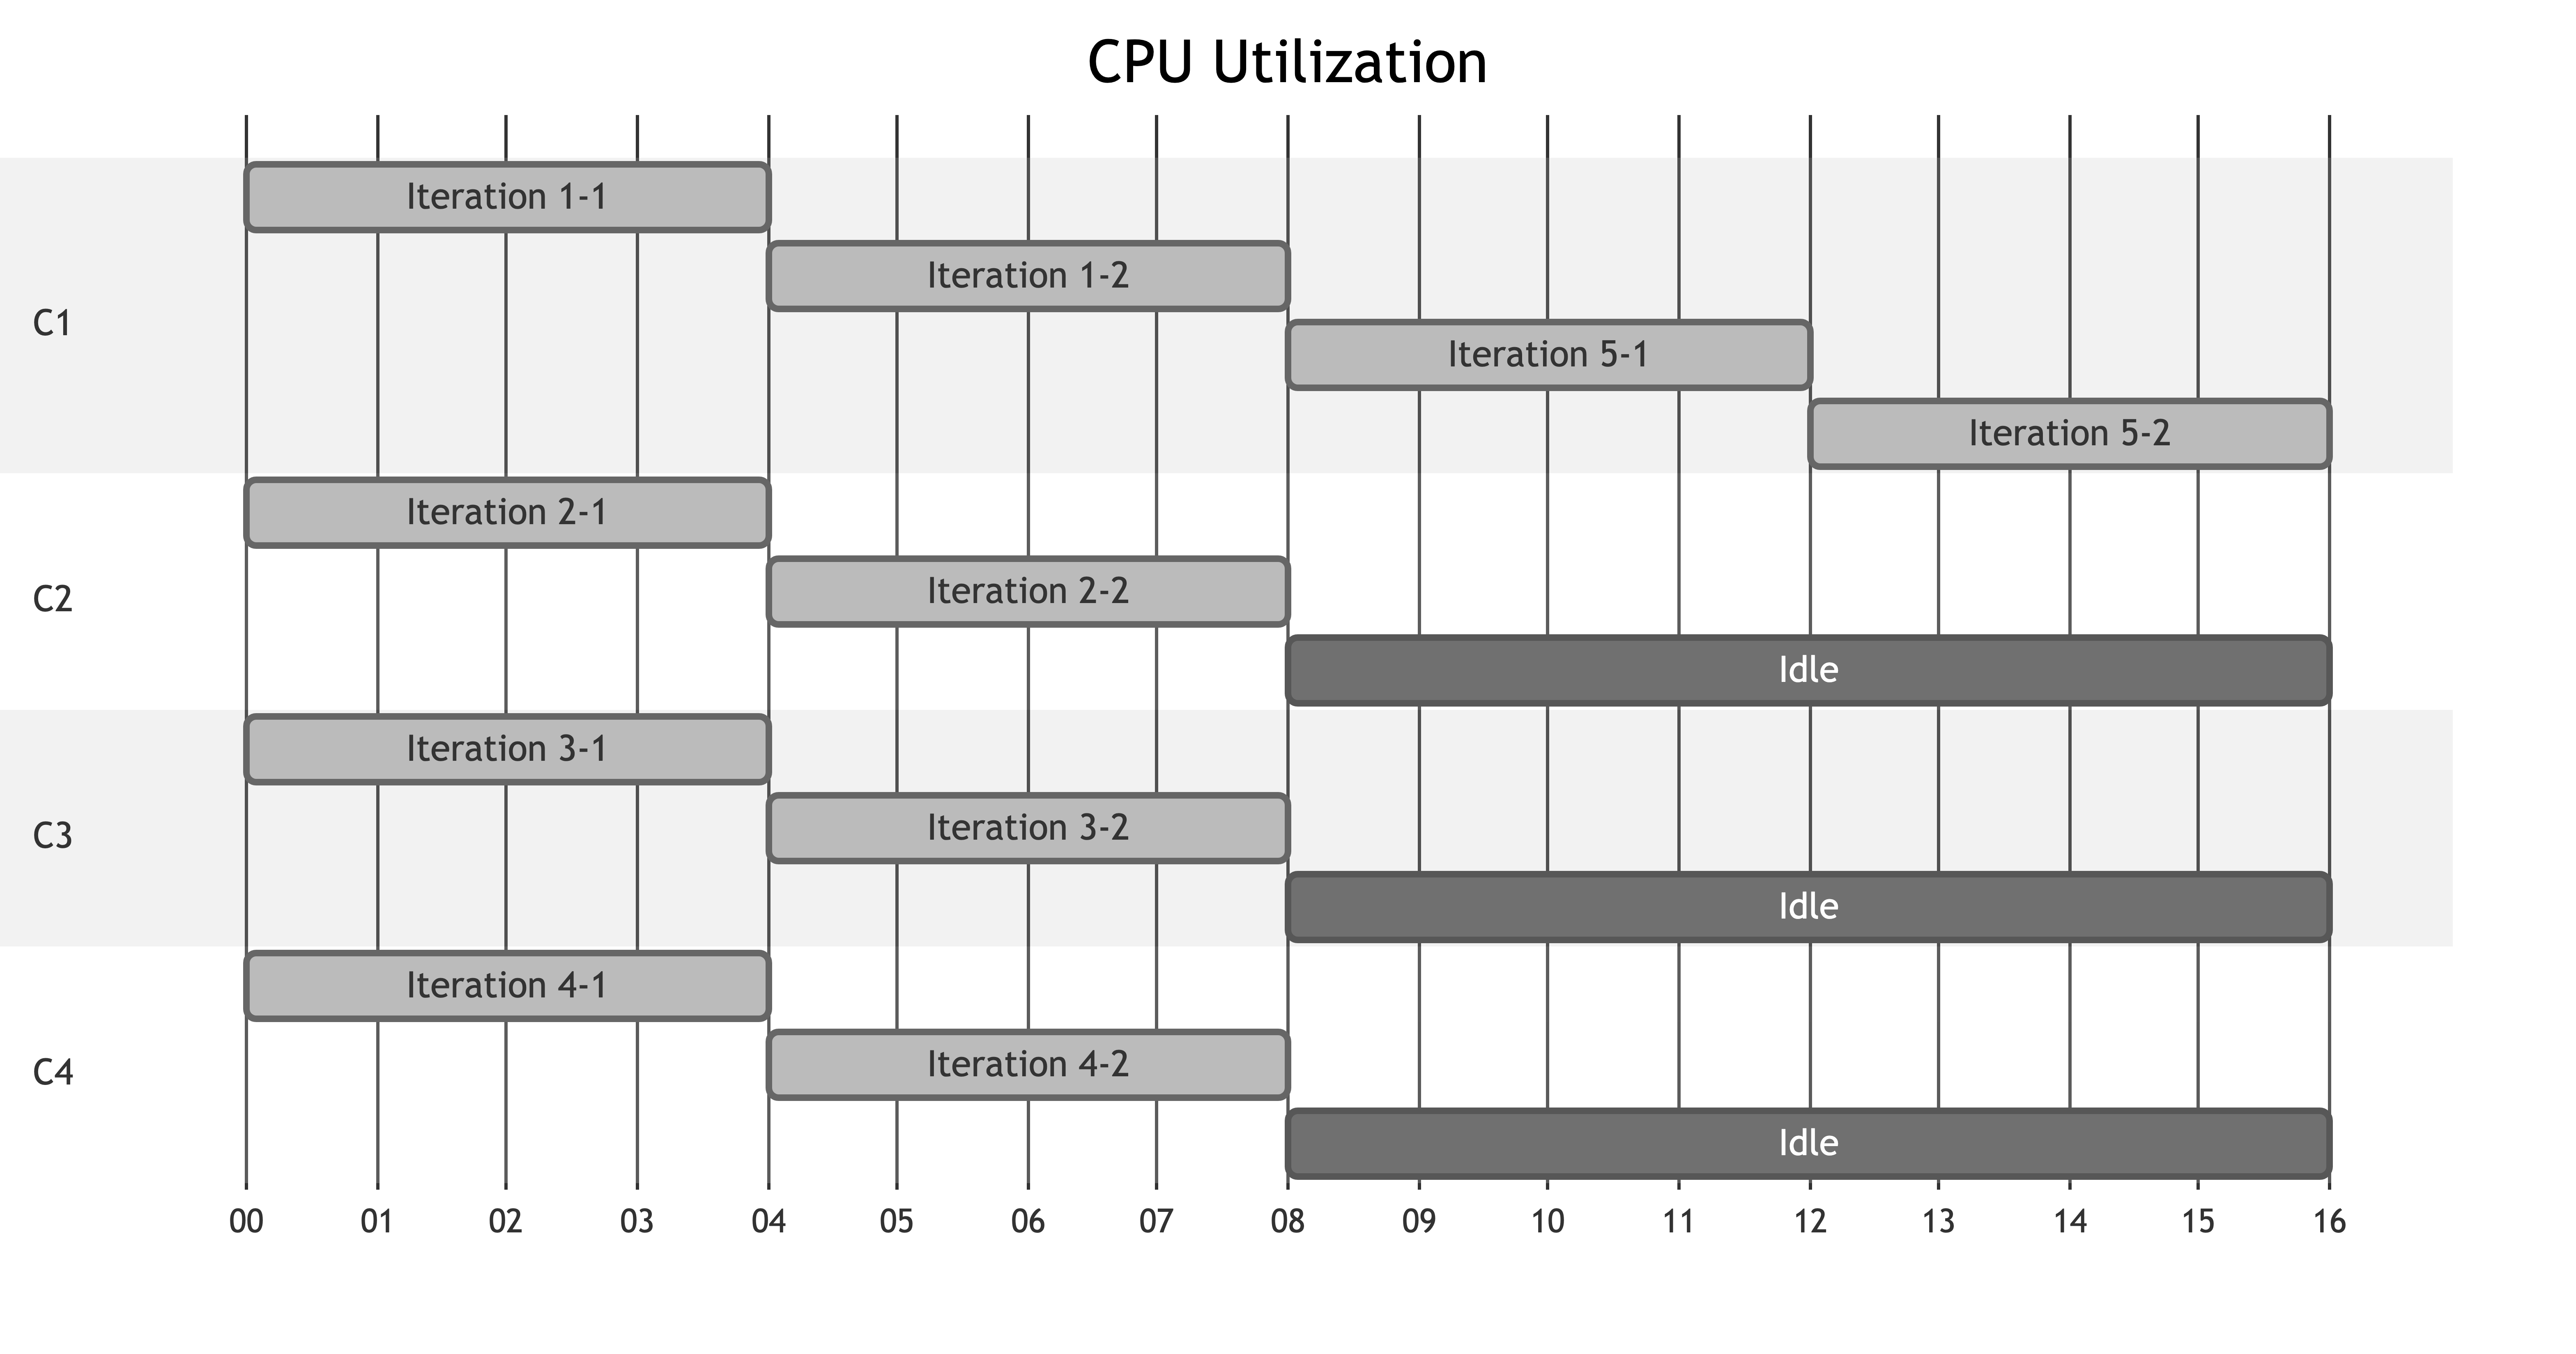
\includegraphics[width=5.5in,height=2.89in]{chapters/chapter10/advanced_technical_aspects_of_mlr3_files/figure-latex/mermaid-figure-1.png}

}

\end{figure}

}

\caption{\label{fig-parallel-outer}CPU utilization for four CPUs while
parallelizing the outer five-fold CV with a sequential two-fold CV
inside. Jobs are labeled as {[}iteration outer{]}-{[}iteration
inner{]}.}

\end{figure}

\begin{figure}

{\centering 

\begin{figure}[H]

{\centering 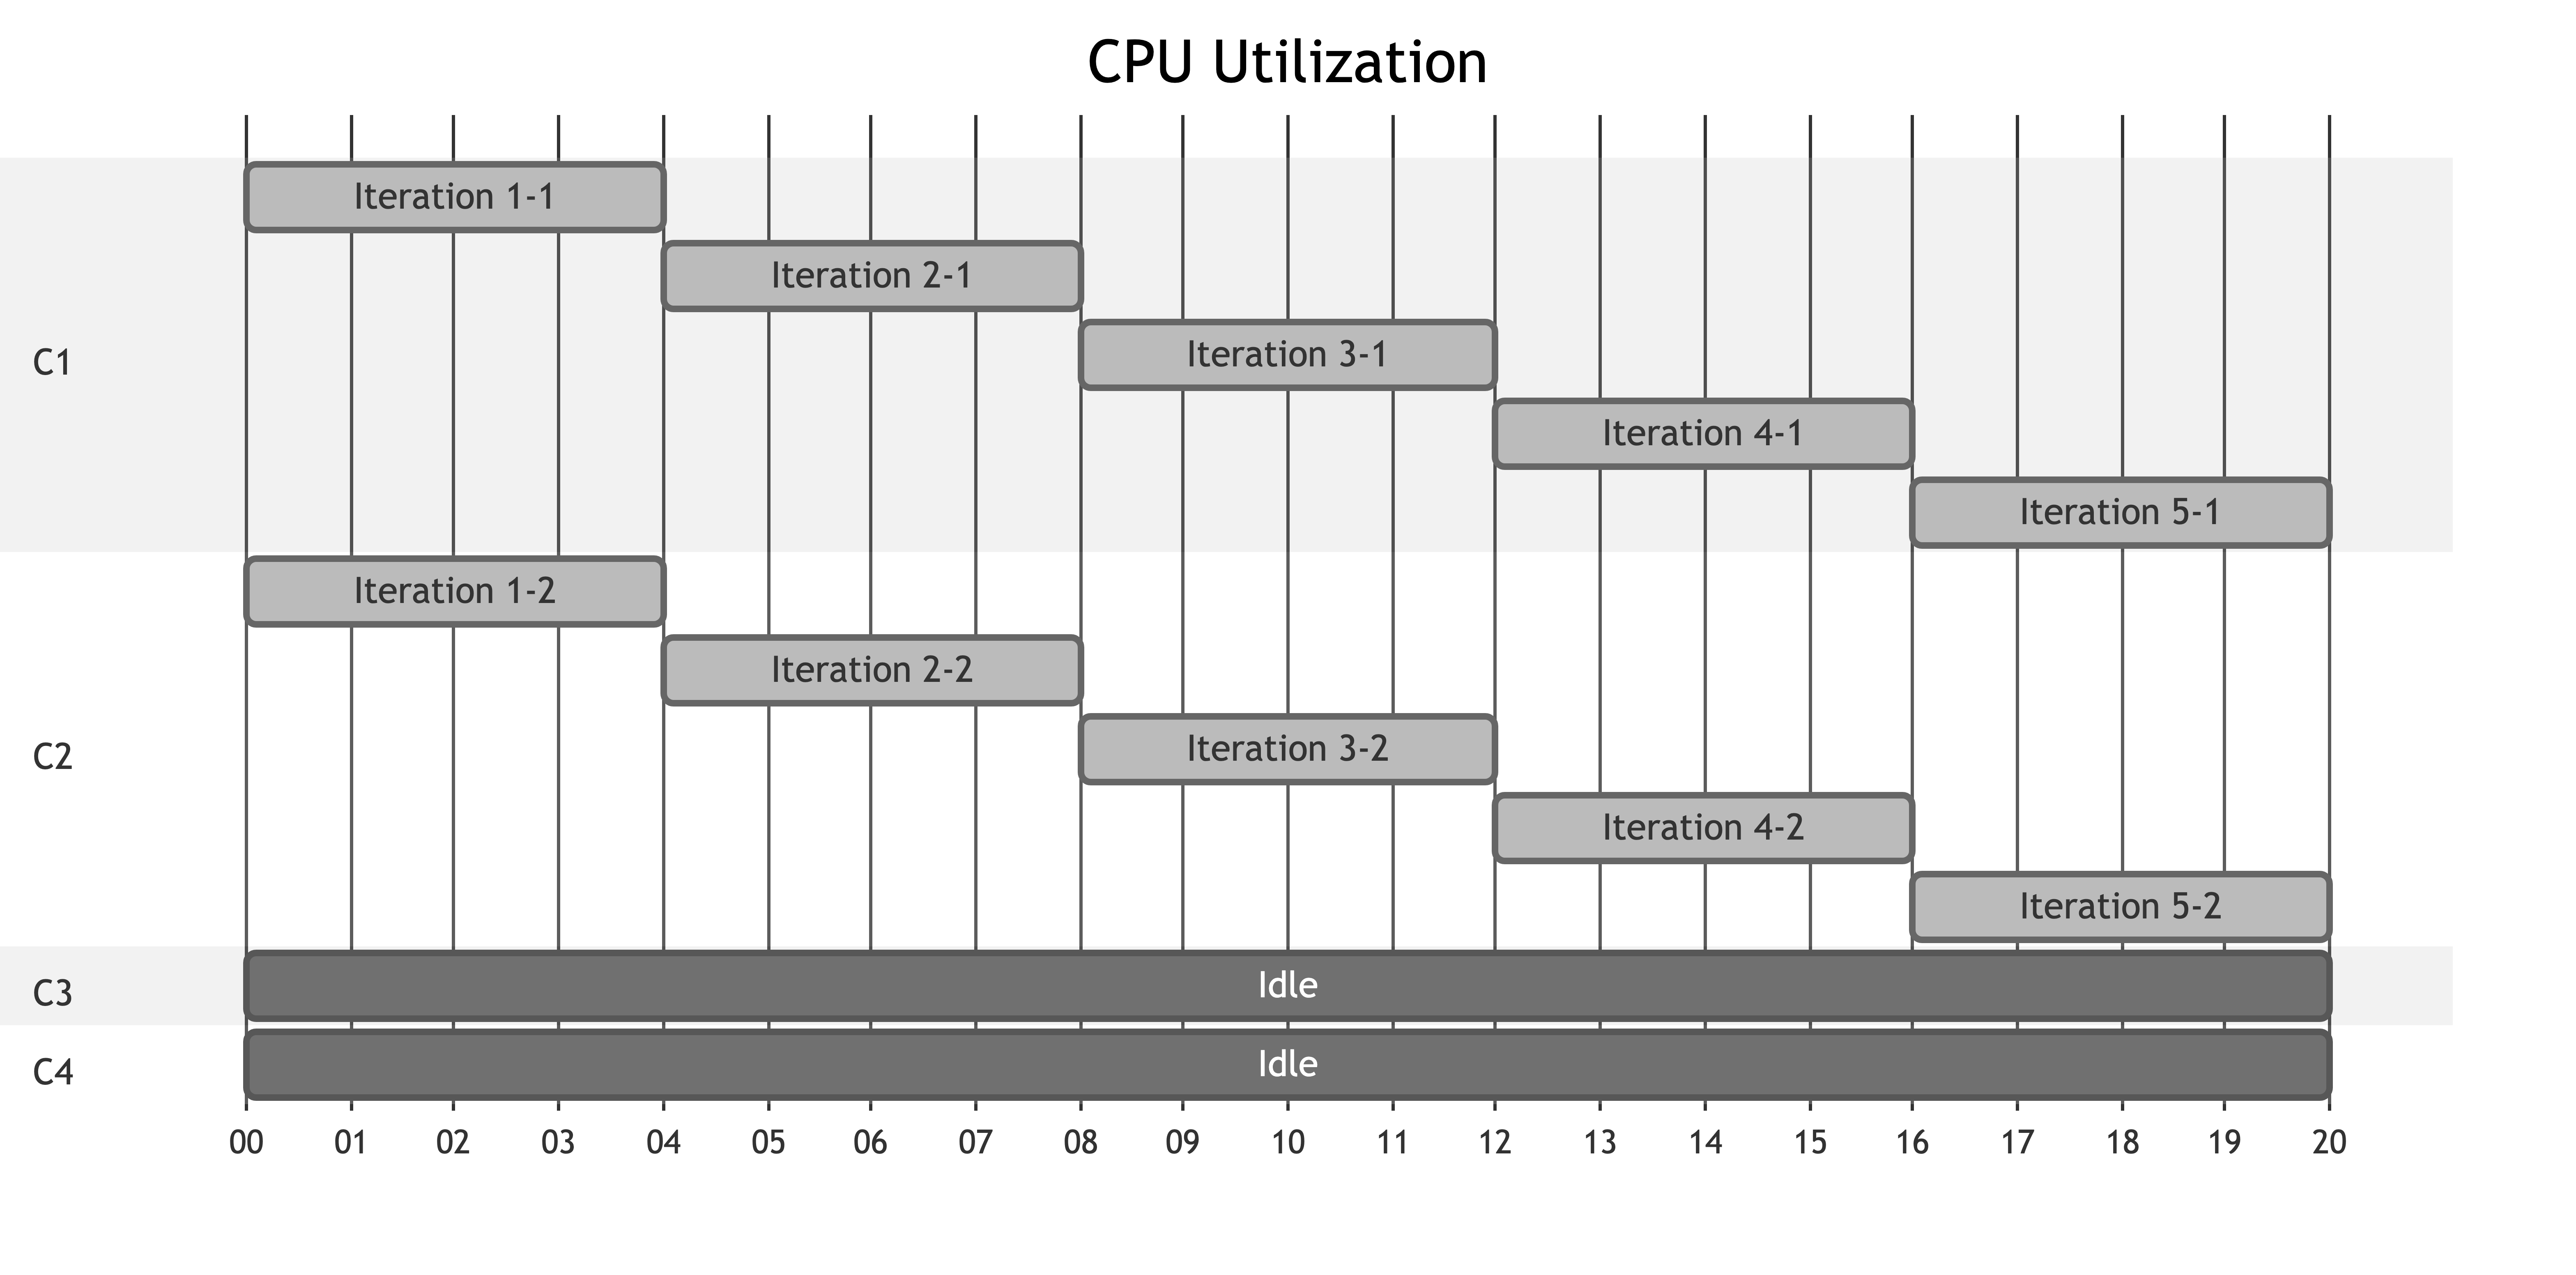
\includegraphics[width=5.5in,height=2.72in]{chapters/chapter10/advanced_technical_aspects_of_mlr3_files/figure-latex/mermaid-figure-2.png}

}

\end{figure}

}

\caption{\label{fig-parallel-inner}CPU utilization for four cores while
parallelizing the inner benchmarking (consisting of two holdout
evaluations) with a sequential five-fold CV outside. Jobs are labeled as
{[}iteration outer{]}-{[}iteration inner{]}.}

\end{figure}

In this example, both possibilities for parallelization are not
exploiting the full potential of the four cores. With parallelization of
the outer loop, all results are computed after 16 seconds, if we
parallelize the inner loop we obtain them after 20 seconds, and in both
cases some CPU cores remain idle for at least some of the time.

\texttt{mlr3} and \texttt{future} make it possible to enable
parallelization for both loops for nested parallelization, even on
different parallelization backends, which can be useful in some
distributed computing setups. Note that the detection of available cores
does not work for such a nested parallelization and the number of
workers must be manually set instead:

\begin{Shaded}
\begin{Highlighting}[]
\CommentTok{\# Runs both loops in parallel}
\NormalTok{future}\SpecialCharTok{::}\FunctionTok{plan}\NormalTok{(}\FunctionTok{list}\NormalTok{(}
  \FunctionTok{tweak}\NormalTok{(}\StringTok{"multisession"}\NormalTok{, }\AttributeTok{workers =} \DecValTok{2}\NormalTok{),}
  \FunctionTok{tweak}\NormalTok{(}\StringTok{"multisession"}\NormalTok{, }\AttributeTok{workers =} \DecValTok{2}\NormalTok{)}
\NormalTok{))}
\end{Highlighting}
\end{Shaded}

This example would run on up to four cores on the local machine: first,
two new sessions would be spawned for the outer loop. Both new sessions
then spawn two additional sessions each to evaluate the inner benchmark.
Although two cores are still idle when the fifth outer resampling
iteration runs, this approach reduces the total runtime to 12 seconds,
which is optimal in this example.

\hypertarget{sec-parallel-predict}{%
\subsection{Parallelization of Predictions}\label{sec-parallel-predict}}

Finally, predictions from a single learner can be parallelized as the
predictions of multiple observations are independent. For most learners,
training is the bottleneck and parallelizing the prediction is not a
worthwhile endeavor, but there can be exceptions, e.g., if your test
dataset is very large.

To predict in parallel, the test data is first split into multiple
groups and the predict method of the learner is applied to each group in
parallel using an active backend configured via
\href{https://www.rdocumentation.org/packages/future/topics/plan}{\texttt{plan()}}.
The resulting predictions are then combined internally in a second step.
To avoid predicting in parallel accidentally, parallel predictions must
be enabled in the learner via the \texttt{parallel\_predict} field:

\begin{Shaded}
\begin{Highlighting}[]
\CommentTok{\# train random forest on sonar task}
\NormalTok{tsk\_sonar }\OtherTok{=} \FunctionTok{tsk}\NormalTok{(}\StringTok{"sonar"}\NormalTok{)}
\NormalTok{lrn\_rpart }\OtherTok{=} \FunctionTok{lrn}\NormalTok{(}\StringTok{"classif.rpart"}\NormalTok{)}
\NormalTok{lrn\_rpart}\SpecialCharTok{$}\FunctionTok{train}\NormalTok{(tsk\_sonar)}

\CommentTok{\# set up parallel predict on four workers}
\NormalTok{future}\SpecialCharTok{::}\FunctionTok{plan}\NormalTok{(}\StringTok{"multisession"}\NormalTok{, }\AttributeTok{workers =} \DecValTok{4}\NormalTok{)}
\NormalTok{lrn\_rpart}\SpecialCharTok{$}\NormalTok{parallel\_predict }\OtherTok{=} \ConstantTok{TRUE}

\CommentTok{\# predict}
\NormalTok{prediction }\OtherTok{=}\NormalTok{ lrn\_rpart}\SpecialCharTok{$}\FunctionTok{predict}\NormalTok{(tsk\_sonar)}
\end{Highlighting}
\end{Shaded}

\hypertarget{sec-error-handling}{%
\section{Error Handling}\label{sec-error-handling}}

In large experiments, it is not uncommon that a model fit or prediction
fails with an error.\index{debugging} This is because the algorithms
have to process arbitrary data, and not all eventualities can always be
handled. While we try to identify obvious problems before execution,
such as when missing values occur for a learner that cannot handle them,
other problems are far more complex to detect. Examples include
numerical problems that may cause issues in training (e.g., due to lack
of convergence), or new levels of categorical variables appearing in the
prediction step. Different learners behave quite differently when
encountering such problems: some models signal a warning during the
training step that they failed to fit but return a baseline model, while
other models stop the execution. During prediction, some learners error
and refuse to predict the response for observations they cannot handle,
while others may predict \texttt{NA}. In this section, we will discuss
how to prevent these errors from causing the program to stop when we do
not want it to (e.g., during a benchmark experiment).

For illustration (and internal testing) of error handling, \texttt{mlr3}
ships with \texttt{lrn("classif.debug")} and \texttt{lrn("regr.debug")}:

\begin{Shaded}
\begin{Highlighting}[]
\NormalTok{tsk\_penguins }\OtherTok{=} \FunctionTok{tsk}\NormalTok{(}\StringTok{"penguins"}\NormalTok{)}
\NormalTok{lrn\_debug }\OtherTok{=} \FunctionTok{lrn}\NormalTok{(}\StringTok{"classif.debug"}\NormalTok{)}
\NormalTok{lrn\_debug}
\end{Highlighting}
\end{Shaded}

\begin{verbatim}
<LearnerClassifDebug:classif.debug>: Debug Learner for Classification
* Model: -
* Parameters: list()
* Packages: mlr3
* Predict Types:  [response], prob
* Feature Types: logical, integer, numeric, character, factor,
  ordered
* Properties: hotstart_forward, missings, multiclass, twoclass
\end{verbatim}

This learner lets us simulate problems that are frequently encountered
in ML. It can be configured to stochastically trigger warnings, errors,
and even segfaults, during training or prediction.

With the learner's default settings, the learner will remember a random
label and constantly predict this label without signaling any
conditions. In the following code we tell the learner to signal an error
during the training step:

\begin{Shaded}
\begin{Highlighting}[]
\CommentTok{\# set probability to signal an error to \textasciigrave{}1\textasciigrave{}}
\NormalTok{lrn\_debug}\SpecialCharTok{$}\NormalTok{param\_set}\SpecialCharTok{$}\NormalTok{values}\SpecialCharTok{$}\NormalTok{error\_train }\OtherTok{=} \DecValTok{1}
\NormalTok{lrn\_debug}\SpecialCharTok{$}\FunctionTok{train}\NormalTok{(tsk\_penguins)}
\end{Highlighting}
\end{Shaded}

\begin{verbatim}
Error in .__LearnerClassifDebug__.train(self = self, private = private, :
	Error from classif.debug->train()
\end{verbatim}

Now we can look at how to deal with errors during \texttt{mlr3}
experiments.

\hypertarget{sec-encapsulation}{%
\subsection{\texorpdfstring{Encapsulation\index{encapsulation}}{Encapsulation}}\label{sec-encapsulation}}

Encapsulation ensures that signaled conditions (e.g., messages, warnings
and errors) are intercepted and that all conditions raised during the
training or prediction step are logged into the learner without
interrupting the program flow. This means that models can be used for
fitting and predicting and any conditions can be analyzed post hoc.
However, the result of the experiment will be a missing model and/or
predictions, depending on where the error occurs. In
Section~\ref{sec-fallback}, we will discuss fallback learners to replace
missing models and/or predictions.

Each
\href{https://mlr3.mlr-org.com/reference/Learner.html}{\texttt{Learner}}
contains the field
\texttt{\$encapsulate}\index{\texttt{Learner}!\texttt{\$encapsulate}}{\marginnote{\begin{footnotesize}\$encapsulate\end{footnotesize}}}
to control how the train or predict steps are wrapped. The first way to
encapsulate the execution is provided by the package
\href{https://cran.r-project.org/package=evaluate}{\texttt{evaluate}},
which evaluates R expressions and captures and tracks conditions
(outputs, messages, warnings or errors) without letting them stop the
process (see documentation of
\href{https://mlr3misc.mlr-org.com/reference/encapsulate.html}{\texttt{encapsulate()}}
for full details):

\begin{Shaded}
\begin{Highlighting}[]
\CommentTok{\# trigger warning and error in training}
\NormalTok{lrn\_debug }\OtherTok{=} \FunctionTok{lrn}\NormalTok{(}\StringTok{"classif.debug"}\NormalTok{, }\AttributeTok{warning\_train =} \DecValTok{1}\NormalTok{, }\AttributeTok{error\_train =} \DecValTok{1}\NormalTok{)}

\CommentTok{\# enable encapsulation for train() and predict()}
\NormalTok{lrn\_debug}\SpecialCharTok{$}\NormalTok{encapsulate }\OtherTok{=} \FunctionTok{c}\NormalTok{(}\AttributeTok{train =} \StringTok{"evaluate"}\NormalTok{, }\AttributeTok{predict =} \StringTok{"evaluate"}\NormalTok{)}
\NormalTok{lrn\_debug}\SpecialCharTok{$}\FunctionTok{train}\NormalTok{(tsk\_penguins)}
\end{Highlighting}
\end{Shaded}

Note how we passed \texttt{"evaluate"} to \texttt{train} and
\texttt{predict} to enable encapsulation in both training and
predicting. However, we could have only set encapsulation for one of
these stages by instead passing
\texttt{c(train\ =\ "evaluate",\ predict\ =\ "none")} or
\texttt{c(train\ =\ "none",\ predict\ =\ "evaluate")}.

Note that encapsulation captures all output written to the standard
output (stdout) and standard error (stderr) streams and stores them in
the learner's log. However, in some computational setups, the calling
process needs to operate on the log output, such as the
\href{https://cran.r-project.org/package=batchtools}{\texttt{batchtools}}
package in Chapter~\ref{sec-large-benchmarking}. In this case, use the
encapsulation method \texttt{"try"} instead, which catches signaled
conditions but does not suppress the output.

After training the learner, one can access the log via the fields
\texttt{log}, \texttt{warnings} and \texttt{errors}:

\begin{Shaded}
\begin{Highlighting}[]
\NormalTok{lrn\_debug}\SpecialCharTok{$}\NormalTok{log}
\end{Highlighting}
\end{Shaded}

\begin{verbatim}
   stage   class                                 msg
1: train warning Warning from classif.debug->train()
2: train   error   Error from classif.debug->train()
\end{verbatim}

\begin{Shaded}
\begin{Highlighting}[]
\NormalTok{lrn\_debug}\SpecialCharTok{$}\NormalTok{warnings}
\end{Highlighting}
\end{Shaded}

\begin{verbatim}
[1] "Warning from classif.debug->train()"
\end{verbatim}

\begin{Shaded}
\begin{Highlighting}[]
\NormalTok{lrn\_debug}\SpecialCharTok{$}\NormalTok{errors}
\end{Highlighting}
\end{Shaded}

\begin{verbatim}
[1] "Error from classif.debug->train()"
\end{verbatim}

Another encapsulation method is implemented in the
\href{https://cran.r-project.org/package=callr}{\texttt{callr}} package.
In contrast to \texttt{evaluate}, the computation is handled in a
separate R process. This guards the calling session against segmentation
faults which otherwise would tear down the complete main R session (if
we demonstrate that here we would break our book). On the downside,
starting new processes comes with comparably more computational
overhead.

\begin{Shaded}
\begin{Highlighting}[]
\NormalTok{lrn\_debug}\SpecialCharTok{$}\NormalTok{encapsulate }\OtherTok{=} \FunctionTok{c}\NormalTok{(}\AttributeTok{train =} \StringTok{"callr"}\NormalTok{, }\AttributeTok{predict =} \StringTok{"callr"}\NormalTok{)}
\CommentTok{\# set segfault\_train and remove warning\_train and error\_train}
\NormalTok{lrn\_debug}\SpecialCharTok{$}\NormalTok{param\_set}\SpecialCharTok{$}\NormalTok{values }\OtherTok{=} \FunctionTok{list}\NormalTok{(}\AttributeTok{segfault\_train =} \DecValTok{1}\NormalTok{)}
\NormalTok{lrn\_debug}\SpecialCharTok{$}\FunctionTok{train}\NormalTok{(}\AttributeTok{task =}\NormalTok{ tsk\_penguins)}\SpecialCharTok{$}\NormalTok{errors}
\end{Highlighting}
\end{Shaded}

\begin{verbatim}
[1] "callr process exited with status -11"
\end{verbatim}

As well as catching errors, we can also set a timeout, in seconds, so
that learners do not run for an indefinite time (e.g., due to failing to
converge) but are terminated after a specified time. This works most
reliably when using \texttt{callr} encapsulation, since the
\texttt{evaluate} method is sometimes not able to interrupt a learner if
it gets stuck in external compiled code. If learners are interrupted,
then this is logged as an error by the encapsulation process. Again, the
timeout can be set separately for training and prediction:

\begin{Shaded}
\begin{Highlighting}[]
\CommentTok{\# near instant timeout for training, no timeout for predict}
\NormalTok{lrn\_debug}\SpecialCharTok{$}\NormalTok{timeout }\OtherTok{=} \FunctionTok{c}\NormalTok{(}\AttributeTok{train =} \FloatTok{1e{-}5}\NormalTok{, }\AttributeTok{predict =} \ConstantTok{Inf}\NormalTok{)}
\NormalTok{lrn\_debug}\SpecialCharTok{$}\FunctionTok{train}\NormalTok{(}\AttributeTok{task =}\NormalTok{ tsk\_penguins)}\SpecialCharTok{$}\NormalTok{errors}
\end{Highlighting}
\end{Shaded}

\begin{verbatim}
[1] "reached elapsed time limit"
\end{verbatim}

With these methods, we can now catch all conditions and post hoc analyze
messages, warnings and errors.

Unfortunately, catching errors and ensuring an upper time limit is only
half the battle. If there are errors during training then we will not
have a trained model to query, or if there are errors during predicting,
then we will not have predictions to analyze:

\begin{Shaded}
\begin{Highlighting}[]
\CommentTok{\# no saved model as there was an error during training}
\FunctionTok{lrn}\NormalTok{(}\StringTok{"classif.debug"}\NormalTok{, }\AttributeTok{error\_train =} \DecValTok{1}\NormalTok{)}\SpecialCharTok{$}\FunctionTok{train}\NormalTok{(tsk\_penguins)}\SpecialCharTok{$}\NormalTok{model}
\end{Highlighting}
\end{Shaded}

\begin{verbatim}
Error in .__LearnerClassifDebug__.train(self = self, private = private, :
	Error from classif.debug->train()
\end{verbatim}

\begin{Shaded}
\begin{Highlighting}[]
\CommentTok{\# saved model}
\NormalTok{lrn\_debug }\OtherTok{=} \FunctionTok{lrn}\NormalTok{(}\StringTok{"classif.debug"}\NormalTok{, }\AttributeTok{error\_predict =} \DecValTok{1}\NormalTok{)}\SpecialCharTok{$}\FunctionTok{train}\NormalTok{(tsk\_penguins)}
\NormalTok{lrn\_debug}\SpecialCharTok{$}\NormalTok{model}
\end{Highlighting}
\end{Shaded}

\begin{verbatim}
$response
[1] "Adelie"

$pid
[1] 13523

$iter
NULL

$id
[1] "09512759-941c-4359-a701-9305513a021b"

attr(,"class")
[1] "classif.debug_model"
\end{verbatim}

\begin{Shaded}
\begin{Highlighting}[]
\CommentTok{\#  but no predictions due to an error during predicting}
\NormalTok{lrn\_debug}\SpecialCharTok{$}\FunctionTok{predict}\NormalTok{(tsk\_penguins)}
\end{Highlighting}
\end{Shaded}

\begin{verbatim}
Error in .__LearnerClassifDebug__.predict(self = self, private = private, :
	Error from classif.debug->predict()
\end{verbatim}

Missing learners and/or predictions are particularly problematic during
automated processes such as resampling, benchmarking, or tuning
(Section~\ref{sec-encapsulation-fallback}), as results cannot be
aggregated properly across iterations. In the next section, we will look
at fallback learners that impute missing models and predictions.

\hypertarget{sec-fallback}{%
\subsection{\texorpdfstring{Fallback
Learners\index{fallback learner}}{Fallback Learners}}\label{sec-fallback}}

Say an error has occurred when training a model in one or more
iterations during resampling, then there are three methods to proceed
with our experiment:

\begin{enumerate}
\def\labelenumi{\arabic{enumi}.}
\tightlist
\item
  Ignore iterations with failures -- This might be the most frequent
  approach in practice, however, it is \textbf{not} statistically sound.
  Say we are trying to evaluate the performance of a model. This model
  might error if in some resampling splits, there are factor levels
  during predicting that were not seen during training, thus leading to
  the model being unable to handle these and erroring. If we discarded
  failed iterations, our model would appear to perform well despite it
  failing to make predictions for an entire class of features.
\item
  Penalize failing learners -- Instead of ignoring failed iterations, we
  could impute the worst possible score (as defined by a given
  \href{https://mlr3.mlr-org.com/reference/Measure.html}{\texttt{Measure}})
  and thereby heavily penalize the learner for failing. However, this
  will often be too harsh for many problems, and for some measures,
  there is no reasonable value to impute.
\item
  Train and predict with a fallback
  learner\index{fallback learner}{\marginnote{\begin{footnotesize}Fallback
  Learner\end{footnotesize}}} -- Instead of imputing with the worst
  possible score, we could train a baseline learner and make predictions
  from this model.
\end{enumerate}

We strongly recommend the final option, which is statistically sound and
can be easily used in any practical experiment. \texttt{mlr3} includes
two baseline learners: \texttt{lrn("classif.featureless")}, which, in
its default configuration, always predicts the majority class, and
\texttt{lrn("regr.featureless")}, which predicts the average response by
default.

To make this procedure convenient during resampling and benchmarking, we
support fitting a baseline (though in theory you could use any
\texttt{Learner}) as a fallback learner\index{fallback learner} by
passing a
\href{https://mlr3.mlr-org.com/reference/Learner.html}{\texttt{Learner}}
to
\texttt{\$fallback}\index{\texttt{Learner}!\texttt{\$fallback}}{\marginnote{\begin{footnotesize}\$fallback\end{footnotesize}}}.
In the next example, we add a classification baseline to our debug
learner, so that when the debug learner errors, \texttt{mlr3} falls back
to the predictions of the featureless learner internally. Note that
while encapsulation is not enabled explicitly, it is automatically
enabled and set to \texttt{"evaluate"} if a fallback learner is added.

\begin{Shaded}
\begin{Highlighting}[]
\NormalTok{lrn\_debug }\OtherTok{=} \FunctionTok{lrn}\NormalTok{(}\StringTok{"classif.debug"}\NormalTok{, }\AttributeTok{error\_train =} \DecValTok{1}\NormalTok{)}
\NormalTok{lrn\_debug}\SpecialCharTok{$}\NormalTok{fallback }\OtherTok{=} \FunctionTok{lrn}\NormalTok{(}\StringTok{"classif.featureless"}\NormalTok{)}

\NormalTok{lrn\_debug}\SpecialCharTok{$}\FunctionTok{train}\NormalTok{(tsk\_penguins)}
\NormalTok{lrn\_debug}
\end{Highlighting}
\end{Shaded}

\begin{verbatim}
<LearnerClassifDebug:classif.debug>: Debug Learner for Classification
* Model: -
* Parameters: error_train=1
* Packages: mlr3
* Predict Types:  [response], prob
* Feature Types: logical, integer, numeric, character, factor,
  ordered
* Properties: hotstart_forward, missings, multiclass, twoclass
* Errors: Error from classif.debug->train()
\end{verbatim}

The learner's log contains the captured error, and although no model is
stored as the error was in training, we can still obtain predictions
from our fallback:

\begin{Shaded}
\begin{Highlighting}[]
\NormalTok{lrn\_debug}\SpecialCharTok{$}\NormalTok{log}
\end{Highlighting}
\end{Shaded}

\begin{verbatim}
   stage class                               msg
1: train error Error from classif.debug->train()
\end{verbatim}

\begin{Shaded}
\begin{Highlighting}[]
\NormalTok{lrn\_debug}\SpecialCharTok{$}\NormalTok{model}
\end{Highlighting}
\end{Shaded}

\begin{verbatim}
NULL
\end{verbatim}

\begin{Shaded}
\begin{Highlighting}[]
\NormalTok{prediction }\OtherTok{=}\NormalTok{ lrn\_debug}\SpecialCharTok{$}\FunctionTok{predict}\NormalTok{(tsk\_penguins)}
\NormalTok{prediction}\SpecialCharTok{$}\FunctionTok{score}\NormalTok{()}
\end{Highlighting}
\end{Shaded}

\begin{verbatim}
classif.ce 
    0.5581 
\end{verbatim}

In the following snippet, we compare the debug learner with a simple
classification tree. We re-parametrize the debug learner to fail in
roughly 50\% of the resampling iterations during the training step:

\begin{Shaded}
\begin{Highlighting}[]
\NormalTok{lrn\_debug }\OtherTok{=} \FunctionTok{lrn}\NormalTok{(}\StringTok{"classif.debug"}\NormalTok{, }\AttributeTok{error\_train =} \FloatTok{0.5}\NormalTok{)}
\NormalTok{lrn\_debug}\SpecialCharTok{$}\NormalTok{fallback }\OtherTok{=} \FunctionTok{lrn}\NormalTok{(}\StringTok{"classif.featureless"}\NormalTok{)}

\NormalTok{aggr }\OtherTok{=} \FunctionTok{benchmark}\NormalTok{(}\FunctionTok{benchmark\_grid}\NormalTok{(}
\NormalTok{  tsk\_penguins,}
  \FunctionTok{list}\NormalTok{(lrn\_debug, }\FunctionTok{lrn}\NormalTok{(}\StringTok{"classif.rpart"}\NormalTok{)),}
  \FunctionTok{rsmp}\NormalTok{(}\StringTok{"cv"}\NormalTok{, }\AttributeTok{folds =} \DecValTok{20}\NormalTok{)))}\SpecialCharTok{$}\FunctionTok{aggregate}\NormalTok{(}\AttributeTok{conditions =} \ConstantTok{TRUE}\NormalTok{)}
\NormalTok{aggr[, .(learner\_id, warnings, errors, classif.ce)]}
\end{Highlighting}
\end{Shaded}

\begin{verbatim}
      learner_id warnings errors classif.ce
1: classif.debug        0     12    0.61944
2: classif.rpart        0      0    0.05523
\end{verbatim}

Even though the debug learner occasionally failed to provide
predictions, we still obtained a statistically sound aggregated
performance value which we can compare to the aggregated performance of
the classification tree. It is also possible to split the benchmark up
into separate
\href{https://mlr3.mlr-org.com/reference/ResampleResult.html}{\texttt{ResampleResult}}
objects which sometimes helps to get more context. E.g., if we only want
to have a closer look into the debug learner, we can extract the errors
from the corresponding resample results:

\begin{Shaded}
\begin{Highlighting}[]
\NormalTok{rr }\OtherTok{=}\NormalTok{ aggr[learner\_id }\SpecialCharTok{==} \StringTok{"classif.debug"}\NormalTok{]}\SpecialCharTok{$}\NormalTok{resample\_result[[1L]]}
\NormalTok{rr}\SpecialCharTok{$}\NormalTok{errors[}\DecValTok{1}\SpecialCharTok{:}\DecValTok{2}\NormalTok{]}
\end{Highlighting}
\end{Shaded}

\begin{verbatim}
   iteration                               msg
1:         2 Error from classif.debug->train()
2:         4 Error from classif.debug->train()
\end{verbatim}

In summary, combining encapsulation and fallback learners makes it
possible to benchmark and tune unreliable or unstable learning
algorithms in a convenient and statistically sound fashion.

\hypertarget{sec-logging}{%
\section{\texorpdfstring{Logging\index{logging}}{Logging}}\label{sec-logging}}

\texttt{mlr3} uses the
\href{https://cran.r-project.org/package=lgr}{\texttt{lgr}} package to
control the verbosity of the output, i.e., to decide how much output is
shown when \texttt{mlr3} operations are run, from suppression of all
non-critical messages to detailed messaging for debugging. In this
section, we will cover how to change logging levels, redirect output,
and finally change the timing of logging feedback.

\texttt{mlr3} uses the following verbosity levels from \texttt{lgr}:

\begin{itemize}
\tightlist
\item
  \texttt{"warn"} -- Only non-breaking warnings are logged
\item
  \texttt{"info"} -- Information such as model runtimes are logged, as
  well as warnings
\item
  \texttt{"debug"} -- Detailed messaging for debugging, as well as
  information and warnings
\end{itemize}

The default log level in \texttt{mlr3} is \texttt{"info"}, this means
that messages are only displayed for messages that are informative or
worse, i.e., \texttt{"info"} and \texttt{"warn"}.

To change the logging threshold you need to retrieve the \texttt{R6}
logger object from \texttt{lgr}, and then call
\texttt{\$set\_threshold()}, for example, to lower the logging threshold
to enable debugging messaging we would change the threshold to
\texttt{"debug"}:

\begin{Shaded}
\begin{Highlighting}[]
\NormalTok{lgr}\SpecialCharTok{::}\FunctionTok{get\_logger}\NormalTok{(}\StringTok{"mlr3"}\NormalTok{)}\SpecialCharTok{$}\FunctionTok{set\_threshold}\NormalTok{(}\StringTok{"debug"}\NormalTok{)}
\end{Highlighting}
\end{Shaded}

Or to suppress all messaging except warnings:

\begin{Shaded}
\begin{Highlighting}[]
\NormalTok{lgr}\SpecialCharTok{::}\FunctionTok{get\_logger}\NormalTok{(}\StringTok{"mlr3"}\NormalTok{)}\SpecialCharTok{$}\FunctionTok{set\_threshold}\NormalTok{(}\StringTok{"warn"}\NormalTok{)}
\end{Highlighting}
\end{Shaded}

\texttt{lgr} comes with a global option called
\texttt{"lgr.default\_threshold"} which can be set via
\texttt{options()} to make your choice permanent across sessions (note
this will affect all packages using \texttt{lgr}), e.g.,
\texttt{options(lgr.default\_threshold\ =\ "info")}.

The packages in \texttt{mlr3} that make use of optimization, i.e.,
\href{https://mlr3tuning.mlr-org.com}{\texttt{mlr3tuning}}\index{\texttt{mlr3tuning}}
or
\href{https://mlr3fselect.mlr-org.com}{\texttt{mlr3fselect}}\index{\texttt{mlr3fselect}},
use the logger of their base package
\href{https://bbotk.mlr-org.com}{\texttt{bbotk}}. This means you could
disable ``info''-logging from the \texttt{mlr3} logger, but keep the
output from \texttt{mlr3tuning}:

\begin{Shaded}
\begin{Highlighting}[]
\NormalTok{lgr}\SpecialCharTok{::}\FunctionTok{get\_logger}\NormalTok{(}\StringTok{"mlr3"}\NormalTok{)}\SpecialCharTok{$}\FunctionTok{set\_threshold}\NormalTok{(}\StringTok{"warn"}\NormalTok{)}
\NormalTok{lgr}\SpecialCharTok{::}\FunctionTok{get\_logger}\NormalTok{(}\StringTok{"bbotk"}\NormalTok{)}\SpecialCharTok{$}\FunctionTok{set\_threshold}\NormalTok{(}\StringTok{"info"}\NormalTok{)}
\end{Highlighting}
\end{Shaded}

By default, output from \texttt{lgr} is printed in the console, however,
you could choose to redirect this to a file in various formats, for
example to a JSON file:

\begin{Shaded}
\begin{Highlighting}[]
\NormalTok{tf }\OtherTok{=} \FunctionTok{tempfile}\NormalTok{(}\StringTok{"mlr3log\_"}\NormalTok{, }\AttributeTok{fileext =} \StringTok{".json"}\NormalTok{)}

\CommentTok{\# get the logger as R6 object}
\NormalTok{logger }\OtherTok{=}\NormalTok{ lgr}\SpecialCharTok{::}\FunctionTok{get\_logger}\NormalTok{(}\StringTok{"mlr"}\NormalTok{)}

\CommentTok{\# add Json appender}
\NormalTok{logger}\SpecialCharTok{$}\FunctionTok{add\_appender}\NormalTok{(lgr}\SpecialCharTok{::}\NormalTok{AppenderJson}\SpecialCharTok{$}\FunctionTok{new}\NormalTok{(tf), }\AttributeTok{name =} \StringTok{"json"}\NormalTok{)}

\CommentTok{\# signal a warning}
\NormalTok{logger}\SpecialCharTok{$}\FunctionTok{warn}\NormalTok{(}\StringTok{"this is a warning from mlr3"}\NormalTok{)}
\end{Highlighting}
\end{Shaded}

\begin{verbatim}
WARN  [15:32:51.496] this is a warning from mlr3
\end{verbatim}

\begin{Shaded}
\begin{Highlighting}[]
\CommentTok{\# print the contents of the file (splitting over two lines)}
\NormalTok{x }\OtherTok{=} \FunctionTok{readLines}\NormalTok{(tf)}
\FunctionTok{cat}\NormalTok{(}\FunctionTok{paste0}\NormalTok{(}\FunctionTok{substr}\NormalTok{(x, }\DecValTok{1}\NormalTok{, }\DecValTok{71}\NormalTok{), }\StringTok{"}\SpecialCharTok{\textbackslash{}n}\StringTok{"}\NormalTok{, }\FunctionTok{substr}\NormalTok{(x, }\DecValTok{72}\NormalTok{, }\FunctionTok{nchar}\NormalTok{(x))))}
\end{Highlighting}
\end{Shaded}

\begin{verbatim}
{"level":300,"timestamp":"2023-07-04 15:32:51","logger":"mlr","caller":
"eval","msg":"this is a warning from mlr3"}
\end{verbatim}

\begin{Shaded}
\begin{Highlighting}[]
\CommentTok{\# remove the appender again}
\NormalTok{logger}\SpecialCharTok{$}\FunctionTok{remove\_appender}\NormalTok{(}\StringTok{"json"}\NormalTok{)}
\end{Highlighting}
\end{Shaded}

See the vignettes in the \texttt{lgr} for more comprehensive examples.

When using parallelization and/or encapsulation, logs may be delayed,
out of order, or, in case of some errors, not present at all. When it is
necessary to have immediate access to log messages, e.g., when
debugging, one may choose to disable \texttt{future} and encapsulation.
To enable `debug mode', set \texttt{options(mlr3.debug\ =\ TRUE)} and
ensure the \texttt{\$encapsulate} slot of learners is set to
\texttt{"none"} (default) or \texttt{"evaluate"}. Debug mode should only
be enabled during debugging and not in production use as it disables
parallelization and leads to unexpected RNG behavior that prevents
reproducibility.

\hypertarget{sec-backends}{%
\section{Data Backends}\label{sec-backends}}

\texttt{Task} objects store their data in an abstract data object, the
\href{https://mlr3.mlr-org.com/reference/DataBackend.html}{\texttt{DataBackend}}.
A data backend\index{data backend} provides a unified API to retrieve
subsets of the data or query information about it, regardless of how the
data is stored on the system. The default backend uses
\href{https://cran.r-project.org/package=data.table}{\texttt{data.table}}
via the
\href{https://mlr3.mlr-org.com/reference/DataBackendDataTable.html}{\texttt{DataBackendDataTable}}
class as a very fast and efficient in-memory database.

While storing the task's data in memory is most efficient for accessing
it for model fitting, there are two major disadvantages:

\begin{enumerate}
\def\labelenumi{\arabic{enumi}.}
\tightlist
\item
  Even if only a small proportion of the data is required, for example
  when doing subsampling, the complete dataset sits in, and consumes,
  memory. This is especially a problem if you work with large tasks or
  many tasks simultaneously, e.g., for
  benchmarking\index{benchmark experiments}.
\item
  During parallelization (Section~\ref{sec-parallelization}), the
  complete data needs to be transferred to the workers which can
  increase the overhead.
\end{enumerate}

To avoid these drawbacks, especially for larger data, it can be
necessary to interface out-of-memory data to reduce the memory
requirements. This way, only the part of the data which is currently
required by the learners will be placed in the main memory to operate
on. There are multiple options to handle this:

\begin{enumerate}
\def\labelenumi{\arabic{enumi}.}
\tightlist
\item
  \href{https://mlr3db.mlr-org.com/reference/DataBackendDplyr.html}{\texttt{DataBackendDplyr}},
  which interfaces the R package
  \href{https://cran.r-project.org/package=dbplyr}{\texttt{dbplyr}},
  extending
  \href{https://cran.r-project.org/package=dplyr}{\texttt{dplyr}} to
  work on many popular SQL\index{SQL} databases like \emph{MariaDB},
  \emph{PostgresSQL}, or \emph{SQLite}.
\item
  \href{https://mlr3db.mlr-org.com/reference/DataBackendDuckDB.html}{\texttt{DataBackendDuckDB}}
  for the \emph{DuckDB\index{DuckDB}} database connected via
  \href{https://cran.r-project.org/package=duckdb}{\texttt{duckdb}},
  which is a fast, zero-configuration alternative to
  SQLite\index{SQLite}.
\item
  \href{https://mlr3db.mlr-org.com/reference/DataBackendDuckDB.html}{\texttt{DataBackendDuckDB}}
  for Parquet\index{Parquet} files. This means the data does not need to
  be converted to DuckDB's native storage format and instead you can
  work directly on directories containing one or multiple files stored
  in the popular Parquet format.
\end{enumerate}

In the following, we will show how to work with each of these choices
using
\href{https://mlr3db.mlr-org.com}{\texttt{mlr3db}}\index{\texttt{mlr3db}}.

\hypertarget{databases-with-databackenddplyr}{%
\subsection{Databases with
DataBackendDplyr}\label{databases-with-databackenddplyr}}

To demonstrate
\href{https://mlr3db.mlr-org.com/reference/DataBackendDplyr.html}{\texttt{DataBackendDplyr}}
we use the (pretty big) NYC flights dataset from the
\href{https://cran.r-project.org/package=nycflights13}{\texttt{nycflights13}}
package and move it into a SQLite\index{SQLite} database. Although
\href{https://mlr3db.mlr-org.com/reference/as_sqlite_backend.html}{\texttt{as\_sqlite\_backend()}}
provides a convenient function to perform this step, we construct the
database manually here.

\begin{Shaded}
\begin{Highlighting}[]
\CommentTok{\# load data}
\FunctionTok{requireNamespace}\NormalTok{(}\StringTok{"DBI"}\NormalTok{)}
\FunctionTok{requireNamespace}\NormalTok{(}\StringTok{"RSQLite"}\NormalTok{)}
\FunctionTok{requireNamespace}\NormalTok{(}\StringTok{"nycflights13"}\NormalTok{)}
\FunctionTok{data}\NormalTok{(}\StringTok{"flights"}\NormalTok{, }\AttributeTok{package =} \StringTok{"nycflights13"}\NormalTok{)}
\FunctionTok{dim}\NormalTok{(flights)}
\end{Highlighting}
\end{Shaded}

\begin{verbatim}
[1] 336776     19
\end{verbatim}

\begin{Shaded}
\begin{Highlighting}[]
\CommentTok{\# add column of unique row ids}
\NormalTok{flights}\SpecialCharTok{$}\NormalTok{row\_id }\OtherTok{=} \FunctionTok{seq}\NormalTok{(}\FunctionTok{nrow}\NormalTok{(flights))}

\CommentTok{\# create sqlite database in temporary file}
\NormalTok{path }\OtherTok{=} \FunctionTok{tempfile}\NormalTok{(}\StringTok{"flights"}\NormalTok{, }\AttributeTok{fileext =} \StringTok{".sqlite"}\NormalTok{)}
\NormalTok{con }\OtherTok{=}\NormalTok{ DBI}\SpecialCharTok{::}\FunctionTok{dbConnect}\NormalTok{(RSQLite}\SpecialCharTok{::}\FunctionTok{SQLite}\NormalTok{(), path)}
\NormalTok{tbl }\OtherTok{=}\NormalTok{ DBI}\SpecialCharTok{::}\FunctionTok{dbWriteTable}\NormalTok{(con, }\StringTok{"flights"}\NormalTok{, }\FunctionTok{as.data.frame}\NormalTok{(flights))}
\NormalTok{DBI}\SpecialCharTok{::}\FunctionTok{dbDisconnect}\NormalTok{(con)}

\CommentTok{\# remove in{-}memory data}
\FunctionTok{rm}\NormalTok{(flights)}
\end{Highlighting}
\end{Shaded}

With the SQLite database stored in file \texttt{path}, we now
re-establish a connection and switch to
\href{https://cran.r-project.org/package=dplyr}{\texttt{dplyr}}/\href{https://cran.r-project.org/package=dbplyr}{\texttt{dbplyr}}
for some essential preprocessing.

\begin{Shaded}
\begin{Highlighting}[]
\CommentTok{\# establish connection}
\NormalTok{con }\OtherTok{=}\NormalTok{ DBI}\SpecialCharTok{::}\FunctionTok{dbConnect}\NormalTok{(RSQLite}\SpecialCharTok{::}\FunctionTok{SQLite}\NormalTok{(), path)}

\CommentTok{\# select the "flights" table}
\FunctionTok{library}\NormalTok{(dplyr)}
\FunctionTok{library}\NormalTok{(dbplyr)}
\NormalTok{tbl }\OtherTok{=} \FunctionTok{tbl}\NormalTok{(con, }\StringTok{"flights"}\NormalTok{)}
\end{Highlighting}
\end{Shaded}

As databases are intended to store large volumes of data, a natural
first step is to subset and filter the data to suitable dimensions.
Therefore, we build up an SQL query in a step-wise fashion using
\texttt{dplyr} verbs and:

\begin{enumerate}
\def\labelenumi{\arabic{enumi}.}
\tightlist
\item
  Select a subset of columns to work on;
\item
  Remove observations where the arrival delay (\texttt{arr\_delay}) has
  a missing value;
\item
  Filter the data to only use every second row (to reduce example
  runtime); and
\item
  Merge factor levels of the feature \texttt{carrier} so infrequent
  carriers are replaced by level ``other''.
\end{enumerate}

\begin{Shaded}
\begin{Highlighting}[]
\CommentTok{\# 1. subset columns}
\NormalTok{keep }\OtherTok{=} \FunctionTok{c}\NormalTok{(}\StringTok{"row\_id"}\NormalTok{, }\StringTok{"year"}\NormalTok{, }\StringTok{"month"}\NormalTok{, }\StringTok{"day"}\NormalTok{, }\StringTok{"hour"}\NormalTok{, }\StringTok{"minute"}\NormalTok{, }\StringTok{"dep\_time"}\NormalTok{,}
  \StringTok{"arr\_time"}\NormalTok{, }\StringTok{"carrier"}\NormalTok{, }\StringTok{"flight"}\NormalTok{, }\StringTok{"air\_time"}\NormalTok{, }\StringTok{"distance"}\NormalTok{, }\StringTok{"arr\_delay"}\NormalTok{)}
\NormalTok{tbl }\OtherTok{=} \FunctionTok{select}\NormalTok{(tbl, }\FunctionTok{all\_of}\NormalTok{(keep))}

\CommentTok{\# 2. filter by missing}
\NormalTok{tbl }\OtherTok{=} \FunctionTok{filter}\NormalTok{(tbl, }\SpecialCharTok{!}\FunctionTok{is.na}\NormalTok{(arr\_delay))}

\CommentTok{\# 3. select every other row}
\NormalTok{tbl }\OtherTok{=} \FunctionTok{filter}\NormalTok{(tbl, row\_id }\SpecialCharTok{\%\%} \DecValTok{2} \SpecialCharTok{==} \DecValTok{0}\NormalTok{)}

\CommentTok{\# 4. merge infrequent carriers}
\NormalTok{infrequent }\OtherTok{=} \FunctionTok{c}\NormalTok{(}\StringTok{"OO"}\NormalTok{, }\StringTok{"HA"}\NormalTok{, }\StringTok{"YV"}\NormalTok{, }\StringTok{"F9"}\NormalTok{, }\StringTok{"AS"}\NormalTok{, }\StringTok{"FL"}\NormalTok{, }\StringTok{"VX"}\NormalTok{, }\StringTok{"WN"}\NormalTok{)}
\NormalTok{tbl }\OtherTok{=} \FunctionTok{mutate}\NormalTok{(tbl, }\AttributeTok{carrier =} \FunctionTok{case\_when}\NormalTok{(}
\NormalTok{  carrier }\SpecialCharTok{\%in\%}\NormalTok{ infrequent }\SpecialCharTok{\textasciitilde{}} \StringTok{"other"}\NormalTok{,}
  \ConstantTok{TRUE} \SpecialCharTok{\textasciitilde{}}\NormalTok{ carrier))}
\end{Highlighting}
\end{Shaded}

Having prepared our data, we can now create a
\href{https://mlr3db.mlr-org.com/reference/DataBackendDplyr.html}{\texttt{DataBackendDplyr}}
and can then query basic information from our new
\href{https://mlr3.mlr-org.com/reference/DataBackend.html}{\texttt{DataBackend}}:

\begin{Shaded}
\begin{Highlighting}[]
\FunctionTok{library}\NormalTok{(mlr3db)}
\NormalTok{backend\_flights }\OtherTok{=} \FunctionTok{as\_data\_backend}\NormalTok{(tbl, }\AttributeTok{primary\_key =} \StringTok{"row\_id"}\NormalTok{)}
\FunctionTok{c}\NormalTok{(}\AttributeTok{nrow =}\NormalTok{ backend\_flights}\SpecialCharTok{$}\NormalTok{nrow, }\AttributeTok{ncol =}\NormalTok{ backend\_flights}\SpecialCharTok{$}\NormalTok{ncol)}
\end{Highlighting}
\end{Shaded}

\begin{verbatim}
  nrow   ncol 
163707     13 
\end{verbatim}

\begin{Shaded}
\begin{Highlighting}[]
\NormalTok{backend\_flights}\SpecialCharTok{$}\FunctionTok{head}\NormalTok{()}
\end{Highlighting}
\end{Shaded}

\begin{verbatim}
   row_id year month day hour minute dep_time arr_time carrier flight
1:      2 2013     1   1    5     29      533      850      UA   1714
2:      4 2013     1   1    5     45      544     1004      B6    725
3:      6 2013     1   1    5     58      554      740      UA   1696
4:      8 2013     1   1    6      0      557      709      EV   5708
5:     10 2013     1   1    6      0      558      753      AA    301
6:     12 2013     1   1    6      0      558      853      B6     71
3 variables not shown: [air_time, distance, arr_delay]
\end{verbatim}

Note that the \texttt{DataBackendDplyr} can only operate on the data we
provided, so does not `know' about the rows and columns we already
filtered out (this is in contrast to using \texttt{\$filter} and
\texttt{\$subset} as in Section~\ref{sec-tasks-mutators}, which only
remove row or column roles and not the rows/columns themselves).

With a backend constructed, we can now use the standard \texttt{mlr3}
API:

\begin{Shaded}
\begin{Highlighting}[]
\NormalTok{tsk\_flights }\OtherTok{=} \FunctionTok{as\_task\_regr}\NormalTok{(backend\_flights, }\AttributeTok{id =} \StringTok{"flights\_sqlite"}\NormalTok{,}
  \AttributeTok{target =} \StringTok{"arr\_delay"}\NormalTok{)}
\NormalTok{rsmp\_sub002 }\OtherTok{=} \FunctionTok{rsmp}\NormalTok{(}\StringTok{"subsampling"}\NormalTok{, }\AttributeTok{ratio =} \FloatTok{0.02}\NormalTok{, }\AttributeTok{repeats =} \DecValTok{3}\NormalTok{)}
\end{Highlighting}
\end{Shaded}

Above we created a regression task by passing a backend as the first
argument and then created a resampling strategy where we will subsample
2\% of the observations three times. In each resampling iteration, only
the required subset of the data is queried from the SQLite database and
passed to our learner:

\begin{Shaded}
\begin{Highlighting}[]
\NormalTok{rr }\OtherTok{=} \FunctionTok{resample}\NormalTok{(tsk\_flights, }\FunctionTok{lrn}\NormalTok{(}\StringTok{"regr.rpart"}\NormalTok{), rsmp\_sub002)}
\NormalTok{measures }\OtherTok{=} \FunctionTok{msrs}\NormalTok{(}\FunctionTok{c}\NormalTok{(}\StringTok{"regr.rmse"}\NormalTok{, }\StringTok{"time\_train"}\NormalTok{, }\StringTok{"time\_predict"}\NormalTok{))}
\NormalTok{rr}\SpecialCharTok{$}\FunctionTok{aggregate}\NormalTok{(measures)}
\end{Highlighting}
\end{Shaded}

\begin{verbatim}
   regr.rmse   time_train time_predict 
     35.9536       0.6997       7.3883 
\end{verbatim}

As we have finished our experiment we can now close our connection,
which we can do by removing the \texttt{tbl} object referencing the
connection and then closing it.

\begin{Shaded}
\begin{Highlighting}[]
\FunctionTok{rm}\NormalTok{(tbl)}
\NormalTok{DBI}\SpecialCharTok{::}\FunctionTok{dbDisconnect}\NormalTok{(con)}
\end{Highlighting}
\end{Shaded}

\hypertarget{parquet-files-with-databackendduckdb}{%
\subsection{Parquet Files with
DataBackendDuckDB}\label{parquet-files-with-databackendduckdb}}

DuckDB\index{DuckDB} databases provide a modern alternative to SQLite,
tailored to the needs of ML. Parquet\index{Parquet} is a popular
column-oriented data storage format supporting efficient compression,
making it far superior to other popular data exchange formats such as
CSV.

Converting a \texttt{data.frame} to DuckDB is possible by passing the
\texttt{data.frame} to convert and the \texttt{path} to store the data
to
\href{https://mlr3db.mlr-org.com/reference/as_duckdb_backend.html}{\texttt{as\_duckdb\_backend()}}.
By example, below we first query the location of an example dataset in a
Parquet file shipped with \texttt{mlr3db} and then convert the resulting
\href{https://mlr3db.mlr-org.com/reference/DataBackendDuckDB.html}{\texttt{DataBackendDuckDB}}
object into a classification task, all without loading the dataset into
memory:

\begin{Shaded}
\begin{Highlighting}[]
\NormalTok{path }\OtherTok{=} \FunctionTok{system.file}\NormalTok{(}\FunctionTok{file.path}\NormalTok{(}\StringTok{"extdata"}\NormalTok{, }\StringTok{"spam.parquet"}\NormalTok{),}
  \AttributeTok{package =} \StringTok{"mlr3db"}\NormalTok{)}
\NormalTok{backend }\OtherTok{=} \FunctionTok{as\_duckdb\_backend}\NormalTok{(path)}
\FunctionTok{as\_task\_classif}\NormalTok{(backend, }\AttributeTok{target =} \StringTok{"type"}\NormalTok{)}
\end{Highlighting}
\end{Shaded}

\begin{verbatim}
<TaskClassif:backend> (4601 x 58)
* Target: type
* Properties: twoclass
* Features (57):
  - dbl (57): address, addresses, all, business, capitalAve,
    capitalLong, capitalTotal, charDollar, charExclamation,
    charHash, charRoundbracket, charSemicolon,
    charSquarebracket, conference, credit, cs, data, direct,
    edu, email, font, free, george, hp, hpl, internet, lab,
    labs, mail, make, meeting, money, num000, num1999, num3d,
    num415, num650, num85, num857, order, original, our, over,
    parts, people, pm, project, re, receive, remove, report,
    table, technology, telnet, will, you, your
\end{verbatim}

Accessing the data internally triggers a query and the required subsets
of data are fetched to be stored in an in-memory \texttt{data.frame}.
After the retrieved data is processed, the garbage collector can release
the occupied memory. The backend can also operate on a folder with
multiple parquet files.

\hypertarget{sec-extending}{%
\section{\texorpdfstring{Extending mlr3 and Defining a New
\texttt{Measure}}{Extending mlr3 and Defining a New Measure}}\label{sec-extending}}

After getting this far in the book you are well on your way to being an
\texttt{mlr3} expert and may even want to add more classes to our
universe. While many classes could be extended, all have a similar
design interface and so, we will only demonstrate how to create a custom
\href{https://mlr3.mlr-org.com/reference/Measure.html}{\texttt{Measure}}.
If you are interested in implementing new learners, \texttt{PipeOp}s, or
tuners, then check out the vignettes in the respective packages:
\href{https://mlr3extralearners.mlr-org.com}{\texttt{mlr3extralearners}}\index{\texttt{mlr3extralearners}},
\href{https://mlr3pipelines.mlr-org.com}{\texttt{mlr3pipelines}}\index{\texttt{mlr3pipelines}},
or
\href{https://mlr3tuning.mlr-org.com}{\texttt{mlr3tuning}}\index{\texttt{mlr3tuning}}.
If you are considering creating a package that adds an entirely new task
type then feel free to contact us for some support via GitHub, email, or
Mattermost. This section assumes good knowledge of \texttt{R6}, see
Section~\ref{sec-r6} for a brief introduction and references to further
resources.

As an example, let us consider a regression measure that scores a
prediction as \texttt{1} if the difference between the true and
predicted values is less than one standard deviation of the truth, or
scores the prediction as \texttt{0} otherwise. In maths this would be
defined as
\(f(y, \hat{y}) = \frac{1}{n} \sum_{i=1}^n \mathbb{I}(|y_i - \hat{y}_i| < \sigma_y)\),
where \(\sigma_y\) is the standard deviation of the truth and
\(\mathbb{I}\) is the indicator function. In code, this measure may be
written as:

\begin{Shaded}
\begin{Highlighting}[]
\NormalTok{threshold\_acc }\OtherTok{=} \ControlFlowTok{function}\NormalTok{(truth, response) \{}
  \FunctionTok{mean}\NormalTok{(}\FunctionTok{ifelse}\NormalTok{(}\FunctionTok{abs}\NormalTok{(truth }\SpecialCharTok{{-}}\NormalTok{ response) }\SpecialCharTok{\textless{}} \FunctionTok{sd}\NormalTok{(truth), }\DecValTok{1}\NormalTok{, }\DecValTok{0}\NormalTok{))}
\NormalTok{\}}

\FunctionTok{threshold\_acc}\NormalTok{(}\FunctionTok{c}\NormalTok{(}\DecValTok{100}\NormalTok{, }\DecValTok{0}\NormalTok{, }\DecValTok{1}\NormalTok{), }\FunctionTok{c}\NormalTok{(}\DecValTok{1}\NormalTok{, }\DecValTok{11}\NormalTok{, }\DecValTok{6}\NormalTok{))}
\end{Highlighting}
\end{Shaded}

\begin{verbatim}
[1] 0.6667
\end{verbatim}

By definition of this measure, its values are bounded in \([0, 1]\)
where a perfect score of \(1\) would mean all predictions are within a
standard deviation of the truth, hence for this measure larger scores
are better.

To use this measure in \texttt{mlr3}, we need to create a new
\href{https://www.rdocumentation.org/packages/R6/topics/R6Class}{\texttt{R6Class}},
which will inherit from \texttt{Measure} and in this case specifically
from
\href{https://mlr3.mlr-org.com/reference/MeasureRegr.html}{\texttt{MeasureRegr}}.
The code for this new measure is in the snippet below, with an
explanation following it. This code chunk can be used as a template for
the majority of performance measures.

\begin{Shaded}
\begin{Highlighting}[]
\NormalTok{MeasureRegrThresholdAcc }\OtherTok{=}\NormalTok{ R6}\SpecialCharTok{::}\FunctionTok{R6Class}\NormalTok{(}\StringTok{"MeasureRegrThresholdAcc"}\NormalTok{,}
  \AttributeTok{inherit =}\NormalTok{ mlr3}\SpecialCharTok{::}\NormalTok{MeasureRegr, }\CommentTok{\# regression measure}
  \AttributeTok{public =} \FunctionTok{list}\NormalTok{(}
    \AttributeTok{initialize =} \ControlFlowTok{function}\NormalTok{() \{ }\CommentTok{\# initialize class}
\NormalTok{      super}\SpecialCharTok{$}\FunctionTok{initialize}\NormalTok{(}
        \AttributeTok{id =} \StringTok{"thresh\_acc"}\NormalTok{, }\CommentTok{\# unique ID}
        \AttributeTok{packages =} \FunctionTok{character}\NormalTok{(), }\CommentTok{\# no package dependencies}
        \AttributeTok{properties =} \FunctionTok{character}\NormalTok{(), }\CommentTok{\# no special properties}
        \AttributeTok{predict\_type =} \StringTok{"response"}\NormalTok{, }\CommentTok{\# measures response prediction}
        \AttributeTok{range =} \FunctionTok{c}\NormalTok{(}\DecValTok{0}\NormalTok{, }\DecValTok{1}\NormalTok{), }\CommentTok{\# results in values between (0, 1)}
        \AttributeTok{minimize =} \ConstantTok{FALSE} \CommentTok{\# larger values are better}
\NormalTok{      )}
\NormalTok{    \}}
\NormalTok{  ),}

  \AttributeTok{private =} \FunctionTok{list}\NormalTok{(}
    \CommentTok{\# define score as private method}
    \AttributeTok{.score =} \ControlFlowTok{function}\NormalTok{(prediction, ...) \{}
      \CommentTok{\# define loss}
\NormalTok{      threshold\_acc }\OtherTok{=} \ControlFlowTok{function}\NormalTok{(truth, response) \{}
        \FunctionTok{mean}\NormalTok{(}\FunctionTok{ifelse}\NormalTok{(}\FunctionTok{abs}\NormalTok{(truth }\SpecialCharTok{{-}}\NormalTok{ response) }\SpecialCharTok{\textless{}} \FunctionTok{sd}\NormalTok{(truth), }\DecValTok{1}\NormalTok{, }\DecValTok{0}\NormalTok{))}
\NormalTok{      \}}
      \CommentTok{\# call loss function}
      \FunctionTok{threshold\_acc}\NormalTok{(prediction}\SpecialCharTok{$}\NormalTok{truth, prediction}\SpecialCharTok{$}\NormalTok{response)}
\NormalTok{    \}}
\NormalTok{  )}
\NormalTok{)}
\end{Highlighting}
\end{Shaded}

\begin{enumerate}
\def\labelenumi{\arabic{enumi}.}
\tightlist
\item
  In the first two lines we name the class, here
  \texttt{MeasureRegrThresholdAcc}, and then state this is a regression
  measure that inherits from \texttt{MeasureRegr}.
\item
  We initialize the class by stating its unique ID is
  \texttt{"thresh\_acc"}, that it does not require any external packages
  (\texttt{packages\ =\ character()}) and that it has no special
  properties (\texttt{properties\ =\ character()}).
\item
  We then pass specific details of the loss function which are: it
  measures the quality of a \texttt{"response"} type prediction, its
  values range between \texttt{(0,\ 1)}, and that the loss is optimized
  as its maximum (\texttt{minimize\ =\ FALSE}).
\item
  Finally, we define the score itself as a private method called
  \texttt{.score} where we pass the predictions to the function we
  defined just above.
\end{enumerate}

Sometimes measures require data from the training set, the task, or the
learner. These are usually complex edge-cases examples, so we will not
go into detail here, for working examples we suggest looking at the code
for
\href{https://mlr3proba.mlr-org.com/reference/MeasureSurvSongAUC.html}{\texttt{MeasureSurvSongAUC}}
and
\href{https://mlr3proba.mlr-org.com/reference/MeasureSurvAUC.html}{\texttt{MeasureSurvAUC}}.
You can also consult the manual page of the \texttt{Measure} for an
overview of other properties and meta-data that can be specified.

Once you have defined your measure you can load it with the \texttt{R6}
constructor (\texttt{\$new()}), or make it available to be constructed
with the \texttt{msr()} sugar function by adding it to the
\href{https://mlr3.mlr-org.com/reference/mlr_measures.html}{\texttt{mlr\_measures}}
dictionary:

\begin{Shaded}
\begin{Highlighting}[]
\NormalTok{tsk\_mtcars }\OtherTok{=} \FunctionTok{tsk}\NormalTok{(}\StringTok{"mtcars"}\NormalTok{)}
\NormalTok{split }\OtherTok{=} \FunctionTok{partition}\NormalTok{(tsk\_mtcars)}
\NormalTok{lrn\_featureless }\OtherTok{=} \FunctionTok{lrn}\NormalTok{(}\StringTok{"regr.featureless"}\NormalTok{)}\SpecialCharTok{$}\FunctionTok{train}\NormalTok{(tsk\_mtcars, split}\SpecialCharTok{$}\NormalTok{train)}
\NormalTok{prediction }\OtherTok{=}\NormalTok{ lrn\_featureless}\SpecialCharTok{$}\FunctionTok{predict}\NormalTok{(tsk\_mtcars, split}\SpecialCharTok{$}\NormalTok{test)}
\NormalTok{prediction}\SpecialCharTok{$}\FunctionTok{score}\NormalTok{(MeasureRegrThresholdAcc}\SpecialCharTok{$}\FunctionTok{new}\NormalTok{())}
\end{Highlighting}
\end{Shaded}

\begin{verbatim}
thresh_acc 
    0.7273 
\end{verbatim}

\begin{Shaded}
\begin{Highlighting}[]
\CommentTok{\# or add to dictionary by passing a unique key to the first argument}
\CommentTok{\#  and the class to the second}
\NormalTok{mlr3}\SpecialCharTok{::}\NormalTok{mlr\_measures}\SpecialCharTok{$}\FunctionTok{add}\NormalTok{(}\StringTok{"regr.thresh\_acc"}\NormalTok{, MeasureRegrThresholdAcc)}
\NormalTok{prediction}\SpecialCharTok{$}\FunctionTok{score}\NormalTok{(}\FunctionTok{msr}\NormalTok{(}\StringTok{"regr.thresh\_acc"}\NormalTok{))}
\end{Highlighting}
\end{Shaded}

\begin{verbatim}
thresh_acc 
    0.7273 
\end{verbatim}

While we only covered how to create a simple regression measure, the
process of adding other classes to our universe is in essence the same:

\begin{enumerate}
\def\labelenumi{\arabic{enumi}.}
\tightlist
\item
  Find the right class to inherit from
\item
  Add methods that:

  \begin{enumerate}
  \def\labelenumii{\alph{enumii})}
  \tightlist
  \item
    Initialize the object with the correct properties
    (\texttt{\$initialize()}).
  \item
    Implement the public and private methods that do the actual
    computation. In the above example, this was the private
    \texttt{\$.score()} method.
  \end{enumerate}
\end{enumerate}

We are always happy to chat and welcome new contributors, please get in
touch if you need assistance in extending \texttt{mlr3}.

\hypertarget{conclusion-8}{%
\section{Conclusion}\label{conclusion-8}}

This chapter covered several advanced topics including parallelization,
error handling, logging, working with databases, and extending the
\texttt{mlr3} universe. For simple use cases, you will probably not need
to know each of these topics in detail, however, we do recommend being
familiar at least with error handling and fallback learners, as these
are essential to preventing even simple experiments being interrupted.
If you are working with large experiments or datasets, then
understanding parallelization, logging, and databases will also be
essential.

We have not covered any of these topics extensively and therefore
recommended the following resources should you want to read more about
these areas. If you are interested to learn more about parallelization
in R, we recommend Schmidberger et al. (2009) and Eddelbuettel (2020).
To find out more about logging, have a read of the vignettes in
\texttt{lgr}, which cover everything from logging to JSON files to
retrieving logged objects for debugging. For an overview of available
DBMS in R, see the CRAN task view on databases at
\url{https://cran.r-project.org/view=Databases}, and in particular the
vignettes of the \texttt{dbplyr} package for DBMS readily available in
\texttt{mlr3}.

\hypertarget{tbl-technical-api}{}
\begin{longtable}[]{@{}
  >{\raggedright\arraybackslash}p{(\columnwidth - 4\tabcolsep) * \real{0.3333}}
  >{\raggedright\arraybackslash}p{(\columnwidth - 4\tabcolsep) * \real{0.3333}}
  >{\raggedright\arraybackslash}p{(\columnwidth - 4\tabcolsep) * \real{0.3333}}@{}}
\caption{\label{tbl-technical-api}Important classes and functions
covered in this chapter with underlying class (if applicable), class
constructor or function, and important class fields and methods (if
applicable).}\tabularnewline
\toprule\noalign{}
\begin{minipage}[b]{\linewidth}\raggedright
Class
\end{minipage} & \begin{minipage}[b]{\linewidth}\raggedright
Constructor/Function
\end{minipage} & \begin{minipage}[b]{\linewidth}\raggedright
Fields/Methods
\end{minipage} \\
\midrule\noalign{}
\endfirsthead
\toprule\noalign{}
\begin{minipage}[b]{\linewidth}\raggedright
Class
\end{minipage} & \begin{minipage}[b]{\linewidth}\raggedright
Constructor/Function
\end{minipage} & \begin{minipage}[b]{\linewidth}\raggedright
Fields/Methods
\end{minipage} \\
\midrule\noalign{}
\endhead
\bottomrule\noalign{}
\endlastfoot
- &
\href{https://www.rdocumentation.org/packages/future/topics/plan}{\texttt{plan()}}
& - \\
- &
\href{https://mlr3.mlr-org.com/reference/set_threads.html}{\texttt{set\_threads()}}
& - \\
- &
\href{https://www.rdocumentation.org/packages/future/topics/tweak}{\texttt{tweak()}}
& - \\
\texttt{Learner} & \texttt{lrn()} & \texttt{\$encapsulate};
\texttt{\$fallback}; \texttt{\$timeout}; \texttt{\$parallel\_predict};
\texttt{\$log} \\
\href{https://www.rdocumentation.org/packages/lgr/topics/Logger}{\texttt{Logger}}
&
\href{https://www.rdocumentation.org/packages/lgr/topics/get_logger}{\texttt{get\_logger}}
& \texttt{\$set\_threshold()} \\
\href{https://mlr3db.mlr-org.com/reference/DataBackendDplyr.html}{\texttt{DataBackendDplyr}}
&
\href{https://mlr3.mlr-org.com/reference/as_data_backend.html}{\texttt{as\_data\_backend}}
& - \\
\href{https://mlr3db.mlr-org.com/reference/DataBackendDuckDB.html}{\texttt{DataBackendDuckDB}}
&
\href{https://mlr3db.mlr-org.com/reference/as_duckdb_backend.html}{\texttt{as\_duckdb\_backend}}
& - \\
\end{longtable}

\hypertarget{exercises-8}{%
\section{Exercises}\label{exercises-8}}

\begin{enumerate}
\def\labelenumi{\arabic{enumi}.}
\tightlist
\item
  Consider the following example where you resample a learner (debug
  learner, sleeps for three seconds during train) on four workers using
  the multisession backend:
\end{enumerate}

\begin{Shaded}
\begin{Highlighting}[]
\NormalTok{tsk\_penguins }\OtherTok{=} \FunctionTok{tsk}\NormalTok{(}\StringTok{"penguins"}\NormalTok{)}
\NormalTok{lrn\_debug }\OtherTok{=} \FunctionTok{lrn}\NormalTok{(}\StringTok{"classif.debug"}\NormalTok{, }\AttributeTok{sleep\_train =} \ControlFlowTok{function}\NormalTok{() }\DecValTok{3}\NormalTok{)}
\NormalTok{rsmp\_cv6 }\OtherTok{=} \FunctionTok{rsmp}\NormalTok{(}\StringTok{"cv"}\NormalTok{, }\AttributeTok{folds =} \DecValTok{6}\NormalTok{)}

\NormalTok{future}\SpecialCharTok{::}\FunctionTok{plan}\NormalTok{(}\StringTok{"multisession"}\NormalTok{, }\AttributeTok{workers =} \DecValTok{4}\NormalTok{)}
\FunctionTok{resample}\NormalTok{(tsk\_penguins, lrn\_debug, rsmp\_cv6)}
\end{Highlighting}
\end{Shaded}

\begin{enumerate}
\def\labelenumi{(\alph{enumi})}
\tightlist
\item
  Assuming you were running this experiment on a computer with four
  CPUs, and that the learner would actually calculate something and not
  just sleep: Would all CPUs be busy for the entire time of this
  calculation?
\item
  Prove your point by measuring the elapsed time, e.g., using
  \href{https://www.rdocumentation.org/packages/base/topics/system.time}{\texttt{system.time()}}.
\item
  What would you change in the setup and why?
\end{enumerate}

\begin{enumerate}
\def\labelenumi{\arabic{enumi}.}
\setcounter{enumi}{1}
\item
  Create a new custom binary classification measure (either using
  methods demonstrated in Section~\ref{sec-extending} or with
  \texttt{msr("classif.costs")}) which scores (``prob''-type)
  predictions. This measure should compute the absolute difference
  between the predicted probability for the positive class and a 0-1
  encoding of the ground truth and then average these values across the
  test set. Test this with \texttt{classif.log\_reg} on
  \texttt{tsk(“sonar”)}.
\item
  ``Tune'' the \texttt{error\_train} hyperparameter of the
  \texttt{classif.debug} learner on a continuous interval from 0 to 1,
  using a simple fallback learner. Tune for 50 iterations using random
  search and holdout resampling. Inspect the resulting archive and find
  out which evaluations resulted in an error, and which did not. Now do
  the same in the interval 0.3 to 0.7. Are your results surprising?
\end{enumerate}
